
% \documentclass[acmtog,screen,nonacm]{acmart}
\documentclass[acmtog,screen]{acmart} % siggraph
% \documentclass[acmtog,nonacm,screen]{acmart} % arxiv
%%
%% \BibTeX command to typeset BibTeX logo in the docs
\AtBeginDocument{%
  \providecommand\BibTeX{{%
    Bib\TeX}}}

\acmSubmissionID{318}

% \setcopyright{cc}
\setcctype{by}
\acmJournal{TOG}
\acmYear{2025} \acmVolume{44} \acmNumber{4} \acmArticle{} \acmMonth{8} \acmPrice{}\acmDOI{10.1145/3731154}
%% These commands are for a PROCEEDINGS abstract or paper.
% \acmConference[Conference acronym 'XX]{Make sure to enter the correct
%   conference title from your rights confirmation emai}{June 03--05,
%   2018}{Woodstock, NY}
%%
%%  Uncomment \acmBooktitle if the title of the proceedings is different
%%  from ``Proceedings of ...''!
%%
%%\acmBooktitle{Woodstock '18: ACM Symposium on Neural Gaze Detection,
%%  June 03--05, 2018, Woodstock, NY}
\acmISBN{978-1-4503-XXXX-X/18/06}

\citestyle{acmauthoryear}

\usepackage[english]{babel}
\usepackage[utf8]{inputenc}
\usepackage{CJKutf8}

%\usepackage{ulem}

%% Meta info
\newcommand{\AUTHORS}{Authors}
\newcommand{\TITLE}{Title}
\newcommand{\KEYWORDS}{Keywords}
\newcommand{\CONFERENCE}{Somewhere}
\newcommand{\COLOR}{yes}
\newcommand{\PAGENUMBERS}{yes} 
\newcommand{\COMMENTS}{yes}
\let\Bbbk\relax
%% Basics 
\usepackage{color,balance,xspace,verbatim,ifthen,engord,unicode}

%% Symbol and Math
\let\Bbbk\relax
\usepackage{gensymb,amsmath,wasysym,marvosym}
\let\Bbbk\relax
\usepackage{newtxmath}
\let\Bbbk\relax
\usepackage{booktabs,colortbl,diagbox,multirow,tabularx,tablefootnote} 
\newcommand{\tabincell}[2]{\begin{tabular}{@{}#1@{}}#2\end{tabular}}
\usepackage{dblfloatfix} % allow the table* to be place at the page bottom

%% Figures
\usepackage{caption}
\usepackage{subcaption} % for subfigure and subtable
\usepackage{graphicx,epsfig,epstopdf,wrapfig}
\graphicspath{{./figures/}}
\DeclareGraphicsExtensions{.pdf,.mps,.png,.jpg,.eps,.PNG,.JPG}
\epstopdfsetup{outdir=./figures/}
% [!ht]: avoid occupy the whole page

%% Algorithms
\usepackage{algorithm,algpseudocode}
\renewcommand{\algorithmicrequire}{\textbf{Input:}} %Use Input in the format of Algorithm
\renewcommand{\algorithmicensure}{\textbf{Output:}}


\hyphenation{op-tical net-works semi-conduc-tor}

%% Url
\usepackage{url}
\def\UrlBreaks{\do\A\do\B\do\C\do\D\do\E\do\F\do\G\do\H\do\I\do\J\do\K\do\L\do\M\do\N\do\O\do\P\do\Q\do\R\do\S\do\T\do\U\do\V\do\W\do\X\do\Y\do\Z\do\[\do\\\do\]\do\^\do\_\do\`\do\a\do\b\do\c\do\d\do\e\do\f\do\g\do\h\do\i\do\j\do\k\do\l\do\m\do\n\do\o\do\p\do\q\do\r\do\s\do\t\do\u\do\v\do\w\do\x\do\y\do\z\do\0\do\1\do\2\do\3\do\4\do\5\do\6\do\7\do\8\do\9\do\.\do\@\do\\\do\/\do\!\do\_\do\|\do\;\do\>\do\]\do\)\do\,\do\?\do\'\do+\do\=\do\#}%


\usepackage{pdfpages}

%% Cross reference
\newcommand{\secref}[1]{\S\ref{#1}}
\newcommand{\figref}[1]{Fig.~\ref{#1}}
\newcommand{\tabref}[1]{Tab.~\ref{#1}}
\newcommand{\eqnref}[1]{Eqn.~\ref{#1}}
%\newcommand{\algref}[1]{Alg.~\ref{#1}}

%% Caption with tigher before and after vertical space
\newcommand{\figcaption}[1]{\vspace{-8mm}\caption{#1}\vspace{-4mm}} 
\newcommand{\mfigcaption}[1]{\vspace{-4mm}\caption{#1}\vspace{-2mm}} 
\newcommand{\tabcaption}[1]{\vspace{1mm}\caption{#1}\vspace{-8mm}}
\newcommand{\mtabcaption}[1]{\vspace{-3mm}\caption{#1}\vspace{-8mm}}

%% Numbers in circles
\usepackage{tikz}
\newcommand{\WoB}[1]{{\small \tikz[baseline=(char.base)]{\node[shape=circle,fill=black,draw,inner sep=0.5pt] (char) {\color{white}#1};}}} % used in text
% used on caption or as fallback plan if tikz is not supported
\newcommand{\sWoB}[1]{$\rlap{\Large{\CIRCLE}}{{\color{white}{\footnotesize \raisebox{0.7 pt}{\hspace{3.3pt}#1}}}}$~} % used in caption
\newcommand{\dWoB}[1]{$\rlap{\Large{\CIRCLE}}{{\color{white}{\scriptsize \raisebox{1 pt}{~#1}}}}$~}
\newcommand*\circled[1]{\tikz[baseline=(char.base)]{\node[shape=circle,draw,inner sep=0.5pt] (char) {#1};}}
%\newcommand{\circled}[1]{\textcircled{\small{#1}}} 

%% Math symbol optimization
\newcommand{\superscript}[1]{\ensuremath{^{\textrm{#1}}}}
\newcommand{\argmax}{\operatornamewithlimits{argmax}}
\def\deg{{\,^{\circ}}\xspace}

%% Supplemental heading
\newcommand{\nosection}[1]{\vspace{3pt}\noindent\textbf{#1}}
\newcommand{\nosubsection}[1]{\vspace{3pt}\noindent$\bullet$\hspace{1mm}\textit{#1}}
\newcommand{\heading}[1]{\vspace{3pt}\noindent\textup{\textbf{#1}}}
\newcommand{\blpara}{\vspace{3pt}\noindent$\bullet$\hspace{1mm}} % +.02in or 0.05
\newcommand{\blnosection}[1]{\vspace{3pt}\noindent$\bullet$\hspace{1mm}{#1}}
\newcommand{\blheading}[1]{\vspace{3pt}\noindent$\bullet$\hspace{1mm}\textup{\textbf{#1}}}
\def\newpara{\vspace{3pt}\noindent}

%% Abbreviation optimization
\def\It{\textit}
\def\Bf{\textbf}
\def\eg{\textit{e.g.,}\hspace{1mm}}
\def\ie{\textit{i.e.,}\hspace{1mm}}
\def\etal{\textit{et al.}\hspace{1mm}}
\def\etc{\textit{etc.}\hspace{1mm}}

%% font wrapper
\usepackage{courier} % produce real \texttt
\newcommand{\code}[1]{\mbox{\texttt{#1}}}
\newcommand{\Mod}[1]{\mbox{\textsf{#1}}} % \textup \textsl \texttt \textsf \textrm
\newcommand{\sw}[1]{\mbox{\textsc{#1}}}
%https://www.sharelatex.com/learn/Code_listing

\usepackage{enumitem}

%% Compact environments
\newenvironment{Itemize}{
	\begin{list}{$\bullet$} {
			\setlength{\itemsep}{0pt}
			\setlength{\parsep}{2pt}
			\setlength{\topsep}{2pt}
			\setlength{\partopsep}{0pt}
			\setlength{\leftmargin}{1.5em} % 1.5
			\setlength{\labelwidth}{1em} % 1
			\setlength{\labelsep}{0.5em} % 0.5
	}}
	{\end{list}}	

\newenvironment{Enumerate}{
	\begin{enumerate}[leftmargin=2em]
		\setlength{\itemsep}{2pt}
		\setlength{\topsep}{2pt}
		\setlength{\partopsep}{0pt}
		\setlength{\parskip}{0pt}}
	{\end{enumerate}}

\newenvironment{Circled}{
	\begin{enumerate}[label=\protect\circled{\arabic*},leftmargin=2em]
		\setlength{\itemsep}{3pt}
		\setlength{\topsep}{0pt}
		\setlength{\partopsep}{0pt}
		\setlength{\parskip}{0pt}}
	{\end{enumerate}}

%% Paper revising
\ifthenelse{\equal{\COMMENTS}{yes}}{
	%% Writing Mode 
	\newcommand{\todo}[1]{\textcolor{red}{\textbf{TODO:} #1}}
        \newcommand{\mc}[1]{\textcolor{cyan}{\textbf{Minchen:} #1}}
        \newcommand{\cmy}[1]{\textcolor{purple}{\textbf{Mengyu:} #1}}
        \newcommand{\lzf}[1]{\textcolor{green}{\textbf{Zhaofeng:} #1}}
	\newcommand{\fyi}[1]{\textcolor{blue}{#1}} %content will be included
	\newcommand{\fye}[1]{\textcolor{red}{#1}}  %content will be excluded
	\newcommand{\remind}[1]{\footnote{\textit{\textcolor{red}{\textbf{Remind:} #1}}}}
	\newcommand{\repl}[2]{\textcolor{red}{#1}\textcolor{blue}{\sout{#2}}} % replacement
	\newcommand{\add}[1]{\textcolor{red}{#1}}
	\newcommand{\del}[1]{\color{blue} {\sout{#1}}}
	%\newcommand{\p}[1]{\noindent\parbox{\columnwidth}{\textcolor{magenta}{\textbf{Point to make:} #1}}\vskip 0.5ex}
	\newcommand{\p}[1]{\vskip 1ex \noindent\colorbox{yellow}{\parbox{\columnwidth}{#1}}\vskip 4pt}
	\newcommand{\note}[1]{\vskip 4ex \noindent\colorbox{yellow}{\parbox{\columnwidth}{#1}}\vskip 6ex} % highlight
	\newcommand{\dc}[1]{\textcolor{red}{\underline{#1}}} % double check % \uwave
	\newcommand{\q}[1]{\vskip 1ex \noindent\colorbox{magenta}{\parbox{\columnwidth}{\textbf{Question:} #1}}\vskip 4pt} 
	\newcommand{\qa}[1]{\hl{\textbf{Answer:} #1}}
	%\newcommand{\qa}[1]{\noindent\colorbox{yellow}{\parbox{\columnwidth}{\textbf{Answer:} #1}}\vskip 2ex} % highlight
}{
	%%Submission Mode
	\newcommand{\todo}[1]{}
	\newcommand{\fyi}[1]{#1}
	\newcommand{\fye}[1]{}
	\newcommand{\remind}[1]{}
	\newcommand{\repl}[2]{#1}
	\newcommand{\add}[1]{#1}
	\newcommand{\del}[1]{}
	\newcommand{\p}[1]{}
	\newcommand{\note}[1]{}
	\newcommand{\dc}[1]{#1}	% Conditional setup for PDF options
\newif\ifnotnewacm % Define the conditional
\notnewacmtrue % Set the conditional to true or false as needed

\newif\ifheadnice % Define the conditional
\headnicetrue % Set it to true or false as needed
	\newcommand{\qm}[1]{#1}
	\newcommand{\q}[1]{}
	\newcommand{\qa}[1]{}	
} 
% Conditional setup for PDF options
\newif\ifnotnewacm % Define the conditional
\notnewacmtrue % Set the conditional to true or false as needed

\newif\ifheadnice % Define the conditional
\headnicetrue % Set it to true or false as needed
%% PDF setup
% \ifnotnewacm
% \ifthenelse{\equal{\COLOR}{yes}}
% {\usepackage[colorlinks]{hyperref}} 		% for colored version 
% {\usepackage[pdfborder={0 0 0}]{hyperref}} 	% for B&W version
% \hypersetup{
% 	plainpages=false,
% 	filecolor=cyan,
% 	linkcolor=red,
% 	citecolor=blue,	
% 	urlcolor=magenta,
% 	pdfauthor={\AUTHORS},
% 	pdftitle={\TITLE},
% 	pdfsubject={\CONFERENCE},
% 	pdfkeywords={\KEYWORDS},
% 	bookmarksopen = {true}	
% }
% \else
% \fi

\ifheadnice
\makeatletter
%\@startsection {NAME}{LEVEL}{INDENT}{BEFORESKIP}{AFTERSKIP}{STYLE}
\renewcommand{\section}{\@startsection{section}{1}{\z@}{-.8ex \@plus -.4ex \@minus -.4ex}{.8ex \@plus .4ex \@minus .4ex}{\normalfont\large\bfseries\MakeTextUppercase}} 
% \normalfont\Large\scshape\bfseries 
\renewcommand{\subsection}{\@startsection{subsection}{2}{\z@}{-.8ex\@plus -.2ex \@minus -.2ex}{.4ex \@plus .2ex \@minus .2ex}{\normalfont\large\rmfamily\bfseries}} 
\renewcommand{\subsubsection}{\@startsection{subsubsection}{2}{\z@}{-.4ex\@plus -.2ex \@minus -.2ex}{.2ex \@plus .2ex \@minus .2ex}{\normalfont\large\slshape}}

%\def\section{\@startsection {section}{1}{\z@}{-.8ex \@plus -.4ex \@minus -.4ex}{.8ex \@plus .4ex \@minus .4ex}{\reset@font\large\bf}}
%\def\subsection{\@startsection{subsection}{2}{\z@}{-.8ex\@plus -.2ex \@minus -.2ex}{.4ex \@plus .2ex \@minus .2ex}{\reset@font\normalsize\bf}} 
%\def\subsubsection{\@startsection{subsubsection}{2}{\z@}{-.8ex\@plus -.2ex \@minus -.2ex}{.4ex \@plus .2ex \@minus .2ex}{\reset@font\normalsize\bf}}

% \normalfont \sffamily \rmfamily \ttfamily
% \slshape  \itshape \scshape \upshape 
% \bfseries \mdseries \lfseries
% https://en.wikibooks.org/wiki/LaTeX/Fonts
\makeatother
\else
\fi

%% Cheating sheet
\begin{comment}

%% font size
%  \tiny, \scriptsize, \footnotesize, \small, \normalsize, \large, \Large, \LARGE, \huge, \Huge

%% Alignment
%  flushleft, center, flushright

%% List
%  itemize, enumerate, description 

%% Quotation
%  quote, quotation, verse, verbatim

%% line break
%  \\, \\*(avoid new page), \newpage, \linebreak[n], \nolinebreak[n], \pagebreak[n], \nopagebreak[n], \sloppy, \fussy (default)

%% dash
%  -, --, ---

%% tilde
%  \~, $\sim$

%% ellipsis
%  \ldots

%% degree: $-30\,^{\circ}\mathrm{C}$

%% \paragraph, \subparagraph{}

%% font
\textrm{...} roman 
\textsf{...} sans serif
\texttt{...} typewriter
\textmd{...} medium 
\textbf{...} bold face
\textup{...} upright 
\textit{...} italic
\textsl{...} slanted 
\textsc{...} Small Caps
\textnormal{...} document font
\end{comment}

%% TBD
\begin{comment}

%% Fonts
\usepackage{lmodern}
\usepackage[T1]{fontenc}
\usepackage{textcomp}
%\usepackage{newtxtext,newtxmath}	% Times/Times-like math symbols
\usepackage{bm}						% bold math; use \bm{} in captions
\usepackage{helvet}					% [scaled=0.92]
\usepackage{courier}
\usepackage{beramono}    			% [scaled=0.83]: more compact, good for code

%\usepackage{floatrow}
% Table float box with bottom caption, box width adjusted to content
%\newfloatcommand{capbtabbox}{table}[][\FBwidth]
\usepackage{blindtext}
\end{comment}


%% Figure template
\begin{comment}

\begin{figure*}%[!ht]
\begin{minipage}{.65\linewidth}
\centering
\begin{subfigure}{0.495\linewidth}
\includegraphics[width=\linewidth]{ph_sd.pdf}
\caption{Internet Throughput}
\label{fig:bm_throughtput_internet}
\end{subfigure}%
\hspace{1pt}
\begin{subfigure}{0.495\linewidth}
\includegraphics[width=\linewidth]{ph_sd.pdf}
\caption{Wireless Throughput}
\label{fig:bm_throughput_wireless}
\end{subfigure}%
\figcaption{Benchmark.}
\label{fig:bm}
\end{minipage}
\begin{minipage}{.34\linewidth}
\centering
\includegraphics[width=\linewidth]{ph_sd.pdf}
\figcaption{Migration}
\label{fig:migration}
\end{minipage}
\end{figure*}

\begin{figure*}[!]
\begin{subfigure}{0.33\linewidth}
\includegraphics[width=\linewidth]{ph_sd.pdf}
\caption{Chunk size}
\label{fig:csize}
\end{subfigure}
\begin{subfigure}{0.33\linewidth}
\includegraphics[width=\linewidth]{ph_sd.pdf}
\caption{Encounter time}
\label{fig:encounter}
\end{subfigure}
\begin{subfigure}{0.33\linewidth}
\includegraphics[width=\linewidth]{ph_sd.pdf}
\caption{Disconnection time}
\label{fig:disconn}
\end{subfigure}
\begin{subfigure}{0.33\linewidth}
\includegraphics[width=\linewidth]{ph_sd.pdf}
\caption{Packet loss rate}
\label{fig:plr}
\end{subfigure}
\begin{subfigure}{0.33\linewidth}
\includegraphics[width=\linewidth]{ph_sd.pdf}
\caption{Wireless bandwidth}
\label{fig:wireless_bw}
\end{subfigure}
\begin{subfigure}{0.33\linewidth}
\includegraphics[width=\linewidth]{ph_sd.pdf}
\caption{Internet latency}
\label{fig:latency}
\end{subfigure}
\figcaption{Performance gain under different environmental parameters.}
\label{fig:para}
\end{figure*}

\begin{figure*}[!]
\begin{minipage}[b]{.33\linewidth}
\centering
\includegraphics[width=\linewidth]{ph_sd.pdf}
\caption{Stage policy.}
\label{fig:migration}
\end{minipage}
\begin{minipage}[b]{.33\linewidth}
\centering
\includegraphics[width=\linewidth]{ph_sd.pdf}
\caption{Handoff policy.}
\label{fig:migration}
\end{minipage}
\begin{minipage}[b]{.33\linewidth}
\centering
\includegraphics[width=\linewidth]{ph_sd.pdf}
\caption{Roam policy.}
\label{fig:migration}
\end{minipage}
\end{figure*}

\begin{figure*}
\begin{minipage}[b]{0.246\linewidth}
\centering
\includegraphics[width=\linewidth]{ph_sd.pdf}
\figcaption{***.} 
\label{fig:**}
\end{minipage}
\begin{minipage}[b]{0.246\linewidth}
\centering
\includegraphics[width=\linewidth]{ph_sd.pdf}
\figcaption{***.} 
\label{fig:**}
\end{minipage}	
\begin{minipage}[b]{0.246\linewidth}
\centering
\includegraphics[width=\linewidth]{ph_sd.pdf}
\figcaption{***.} 
\label{fig:**}
\end{minipage}
\begin{minipage}[b]{0.246\linewidth}
\centering
\includegraphics[width=\linewidth]{ph_sd.pdf}
\figcaption{***.} 
\label{fig:**}
\end{minipage}
\end{figure*}

\begin{figure*}
\begin{minipage}[b]{0.33\linewidth}
\centering
\includegraphics[width=\linewidth]{ph_sd.pdf}
\figcaption{***.} 
\label{fig:**}
\end{minipage}
\begin{minipage}[b]{0.33\linewidth}
\centering
\includegraphics[width=\linewidth]{ph_sd.pdf}
\figcaption{***.} 
\label{fig:**}
\end{minipage}	
\begin{minipage}[b]{0.33\linewidth}
\centering
\includegraphics[width=\linewidth]{ph_sd.pdf}
\figcaption{***.} 
\label{fig:**}
\end{minipage}
\end{figure*}

\begin{figure}
\begin{minipage}[b]{0.495\linewidth}
\centering
\includegraphics[width=\linewidth]{ph_sd.pdf}
\figcaption{***.} 
\label{fig:**}
\end{minipage}
\begin{minipage}[b]{0.495\linewidth}
\centering
\includegraphics[width=\linewidth]{ph_sd.pdf}
\figcaption{***.} 
\label{fig:**}
\end{minipage}	
\end{figure}

\begin{figure*}
\begin{minipage}[b]{0.65\linewidth}
\centering	
\subfigure[]{\includegraphics[width=0.49\linewidth]{ph_sd.pdf}} 
\subfigure[]{\includegraphics[width=0.49\linewidth]{ph_sd.pdf}} 
\figcaption{***.}
\label{fig:**}
\end{minipage}
\begin{minipage}[b]{0.345\linewidth}
\centering
\includegraphics[width=\linewidth]{ph_sd.pdf}
\figcaption{***.} 
\label{fig:**}
\end{minipage}	
\end{figure*}

% 1,1,3*1


\end{comment}

%% Table template
\begin{comment}


\end{comment}


%% Chinese template
\begin{comment}
\documentclass[a4paper, 11pt]{article}

%%%%%% 导入包 %%%%%%
\usepackage{CJKutf8}
\usepackage{graphicx}
\usepackage[unicode]{hyperref}
\usepackage{xcolor}
\usepackage{cite}
\usepackage{indentfirst}

%%%%%% 设置字号 %%%%%%
\newcommand{\chuhao}{\fontsize{42pt}{\baselineskip}\selectfont}
\newcommand{\xiaochuhao}{\fontsize{36pt}{\baselineskip}\selectfont}
\newcommand{\yihao}{\fontsize{28pt}{\baselineskip}\selectfont}
\newcommand{\erhao}{\fontsize{21pt}{\baselineskip}\selectfont}
\newcommand{\xiaoerhao}{\fontsize{18pt}{\baselineskip}\selectfont}
\newcommand{\sanhao}{\fontsize{15.75pt}{\baselineskip}\selectfont}
\newcommand{\sihao}{\fontsize{14pt}{\baselineskip}\selectfont}
\newcommand{\xiaosihao}{\fontsize{12pt}{\baselineskip}\selectfont}
\newcommand{\wuhao}{\fontsize{10.5pt}{\baselineskip}\selectfont}
\newcommand{\xiaowuhao}{\fontsize{9pt}{\baselineskip}\selectfont}
\newcommand{\liuhao}{\fontsize{7.875pt}{\baselineskip}\selectfont}
\newcommand{\qihao}{\fontsize{5.25pt}{\baselineskip}\selectfont}

%%%% 设置属性 %%%%
\makeatletter
\renewcommand\section{\@startsection{section}{1}{\z@}%
{-1.5ex \@plus -.5ex \@minus -.2ex}%
{.5ex \@plus .1ex}%
{\normalfont\sihao\CJKfamily{hei}}}
\makeatother

%%%% 设置 subsection 属性 %%%%
\makeatletter
\renewcommand\subsection{\@startsection{subsection}{1}{\z@}%
{-1.25ex \@plus -.5ex \@minus -.2ex}%
{.4ex \@plus .1ex}%
{\normalfont\xiaosihao\CJKfamily{hei}}}
\makeatother

%%%% 设置 subsubsection 属性 %%%%
\makeatletter
\renewcommand\subsubsection{\@startsection{subsubsection}{1}{\z@}%
{-1ex \@plus -.5ex \@minus -.2ex}%
{.3ex \@plus .1ex}%
{\normalfont\xiaosihao\CJKfamily{hei}}}
\makeatother

%%%% 段落首行缩进两个字 %%%%
\makeatletter
\let\@afterindentfalse\@afterindenttrue
\@afterindenttrue
\makeatother
\setlength{\parindent}{2em}  %中文缩进两个汉字位


%%%% 下面的命令重定义页面边距,使其符合中文刊物习惯 %%%%
\addtolength{\topmargin}{-54pt}
\setlength{\oddsidemargin}{0.63cm}  % 3.17cm - 1 inch
\setlength{\evensidemargin}{\oddsidemargin}
\setlength{\textwidth}{14.66cm}
\setlength{\textheight}{24.00cm}    % 24.62

%%%% 下面的命令设置行间距与段落间距 %%%%
\linespread{1.4}
% \setlength{\parskip}{1ex}
\setlength{\parskip}{0.5\baselineskip}

%%%% 正文开始 %%%%
\begin{document}
\begin{CJK}{UTF8}{gbsn}

%%%% 定理类环境的定义 %%%%
\newtheorem{example}{例}             % 整体编号
\newtheorem{algorithm}{算法}
\newtheorem{theorem}{定理}[section]  % 按 section 编号
\newtheorem{definition}{定义}
\newtheorem{axiom}{公理}
\newtheorem{property}{性质}
\newtheorem{proposition}{命题}
\newtheorem{lemma}{引理}
\newtheorem{corollary}{推论}
\newtheorem{remark}{注解}
\newtheorem{condition}{条件}
\newtheorem{conclusion}{结论}
\newtheorem{assumption}{假设}

%%%% 重定义 %%%%
\renewcommand{\contentsname}{目录}  % 将Contents改为目录
\renewcommand{\abstractname}{摘要}  % 将Abstract改为摘要
\renewcommand{\refname}{参考文献}   % 将References改为参考文献
\renewcommand{\indexname}{索引}
\renewcommand{\figurename}{图}
\renewcommand{\tablename}{表}
\renewcommand{\appendixname}{附录}
\renewcommand{\algorithm}{算法}


%%%% 定义标题格式,包括title,author,affiliation,email等 %%%%
\title{***}
\author{***footnote{电子邮件:**}\\[2ex]
*** \\[2ex]
}
\date{20XX年X月}


%%%% 以下部分是正文 %%%%  
\maketitle

\tableofcontents
\newpage
在此输入正文,中英文均可。

\songti 
\fangsong 
\biaosong
\heiti
\kaishu

\end{CJK}
\end{document}
\end{comment}

%%
%% end of the preamble, start of the body of the document source.
\begin{document}

%%
%% The "title" command has an optional parameter,
%% allowing the author to define a "short title" to be used in page headers.
\title{VR-Doh: Hands-on 3D Modeling in Virtual Reality}

\author{Zhaofeng Luo}
\authornote{Both authors contributed equally to this research.}
\affiliation{%
  \institution{Carnegie Mellon University}
  \country{USA}
}
\affiliation{%
  \institution{Peking University}
  \country{China}
}
\email{roushelfy@stu.pku.edu.cn}

\author{Zhitong Cui}
\authornotemark[1]
\affiliation{%
  \institution{Carnegie Mellon University}
  \country{USA}
}
\affiliation{%
  \institution{Zhejiang University}
  \country{China}
}
\email{zhitongcui@zju.edu.cn}

\author{Shijian Luo}
\affiliation{%
  \institution{Zhejiang University}
  \country{China}
}
\email{sjluo@zju.edu.cn}

\author{Mengyu Chu}
\affiliation{%
  \institution{Peking University, State Key Lab of General AI}
  \country{China}
}
\email{mchu@pku.edu.cn}

\author{Minchen Li}
\affiliation{%
  \institution{Carnegie Mellon University}
  \country{USA}
}
\email{minchernl@gmail.com}

% \renewcommand{\shortauthors}{Luo and Cui et al.}

\begin{abstract}
  We introduce VR-Doh, an open-source, hands-on 3D modeling system that enables intuitive creation and manipulation of elastoplastic objects in Virtual Reality (VR). By customizing the Material Point Method (MPM) for real-time simulation of hand-induced large deformations and enhancing 3D Gaussian Splatting for seamless rendering, VR-Doh provides an interactive and immersive 3D modeling experience. Users can naturally sculpt, deform, and edit objects through both contact- and gesture-based hand-object interactions.
  To achieve real-time performance, our system incorporates localized simulation techniques, particle-level collision handling, and the decoupling of physical and appearance representations, ensuring smooth and responsive interactions. VR-Doh supports both object creation and editing, enabling diverse modeling tasks such as designing food items, characters, and interlocking structures, all resulting in simulation-ready assets. User studies with both novice and experienced participants highlight the system's intuitive design, immersive feedback, and creative potential. Compared to existing geometric modeling tools, VR-Doh offers enhanced accessibility and natural interaction, making it a powerful tool for creative exploration in VR.
\end{abstract}

%%
%% The code below is generated by the tool at http://dl.acm.org/ccs.cfm.
%% Please copy and paste the code instead of the example below.
%%
\begin{CCSXML}
<ccs2012>
   <concept>
       <concept_id>10010147.10010371.10010387.10010866</concept_id>
       <concept_desc>Computing methodologies~Virtual reality</concept_desc>
       <concept_significance>500</concept_significance>
       </concept>
   % <concept>
   %     <concept_id>10010147.10010371.10010396.10010400</concept_id>
   %     <concept_desc>Computing methodologies~Point-based models</concept_desc>
   %     <concept_significance>300</concept_significance>
   %     </concept>
 </ccs2012>
\end{CCSXML}

\ccsdesc[500]{Computing methodologies~Virtual reality}
% \ccsdesc[300]{Computing methodologies~Point-based models}

%%
%% Keywords. The author(s) should pick words that accurately describe
%% the work being presented. Separate the keywords with commas.
\keywords{Virtual Reality, 3D Modeling, Elastoplasticity Simulation, Material Point Method, Human-Computer Interaction}
%% A "teaser" image appears between the author and affiliation
%% information and the body of the document, and typically spans the
%% page.

% \received{20 February 2007}
% \received[revised]{12 March 2009}
% \received[accepted]{5 June 2009}

%%
%% This command processes the author and affiliation and title
%% information and builds the first part of the formatted document.


\begin{teaserfigure}
    \centering
    \noindent\includegraphics[width=\linewidth]{img/VR-Doh-Teaser.pdf}
    \caption{The figure demonstrates the intuitive and versatile capabilities of our VR-Doh system. In the upper row, users deform the vase and refine the roses with tools and gestures. The lower row showcases the system's versatility, enabling seamless table deformation by hand contact, object removal, and vase placement. This workflow simplifies complex editing tasks, delivering realistic results efficiently and intuitively.
    %Top row: The vase is deformed using the VR-Doh system through contact-based hand-object interactions, followed by merging a bouquet of roses into the vase. Hand gestures are then used to bend and refine the roses, a process repeated across three stems. Bottom row: The garden scene is edited by removing the original vase, deforming the table with tools, and placing the newly decorated vase with roses as the centerpiece.
    }
  \label{fig:1-teaser}
  % \Description{}
\end{teaserfigure}

\maketitle

\section{Introduction}
% \cmy{We can emphasize the novelty of physics-based modeling with regard to geometry-based modeling. The latter is widely seen in commercial tools but often requires careful observation of real-life objects and specialized expertise to get familiar with the tools, and to learn how to fine-tune and adjust.
% In contrast, physics-based modeling aligns more closely with human intuition and natural interactions:
% 1. Provides a wide range of tools that users can easily use without learning.
% 2. Users can predict the results of their actions very well according to their daily experience, reducing the need for extensive professional experience.
% 3. Offers modeling potential on par with geometry-based approaches, as evidenced by the diversity of the real world.}

With the growing demand for digital content, there is an urgent need to address key challenges in 3D content creation: ease of use, scalability, efficiency, and quality. Traditional 3D modeling tools impose significant barriers for novice users, requiring expertise in real-world observation, specialized techniques, and iterative fine-tuning. This reliance on professional skills limits accessibility, hindering wider participation in high-quality content creation.
% As the demand for digital content continues to grow, there is an increasing need for ease of use, greater quantity, improved efficiency, and higher quality in 3D content creation. Traditional 3D modeling tools impose significant barriers to entry for novice users. These tools often require careful observation of real-world objects, mastery of specialized techniques, and iterative fine-tuning to achieve the desired outcome. This reliance on professional expertise limits accessibility for broader audiences in high-quality content creation.

Meanwhile, 3D modeling in Virtual Reality (VR) has become increasingly popular due to its ability to provide immersion and depth, thereby enhancing designers' creativity and collaboration~\cite{rosales2019surfacebrush, yu2021cassie}. Commercial tools like Shapelab~\cite{shape-lab-no-date}
% \footnote{\url{https://shapelabvr.com/}} \footnote{\url{https://gravitysketch.com/}} 
and Gravity Sketch~\cite{gravity-sketch-no-date} have advanced this vision. However, their approaches are still limited to procedural methods, such as drawing curves to form surfaces from scratch, which are restricted to geometric techniques and require significant skills. 

In contrast, physics-aware shape modeling introduces a novel paradigm that aligns more closely with human intuition and natural interactions. In this approach, objects are simulated as deformable solids, reshaped through contact forces or boundary conditions specified by the user~\cite{Fang2021IDP}. In the context of VR, using hands as an input modality is particularly compelling, as it mimics the way users naturally manipulate physical objects, such as clay. This approach leverages users' prior experience with creating real-world objects, making the modeling process more intuitive and accessible~\cite{schulz2019rodmesh, arora2019magicalhands, pihuit2008hands}.

Building on these foundational advantages, we integrate physics-based simulation into VR to deliver an intuitive and efficient hands-on 3D modeling system, \textit{VR-Doh}. Our primary objective is to enable users to create and edit virtual objects with a high degree of realism, leveraging direct hand-based contact and gestures alongside interactive feedback. To efficiently support large deformations and contact handling, we adopt the Material Point Method (MPM) \cite{jiang2016material, hu2018moving}, a hybrid Lagrangian-Eulerian framework capable of simulating versatile elastoplastic materials.

VR-Doh enables users to create 3D models by deforming and composing built-in primitive geometries, with surface meshes reconstructed from MPM particles. Additionally, based on \citet{xie2024physgaussian}, we extend support for editing existing 3D data represented by Gaussian Splatting (GS)~\cite{kerbl20233d}, allowing content creation through the modification of realistically rendered objects captured from the real world. To achieve real-time responsiveness despite the computational demands of simulation and rendering, we introduce optimizations such as particle-level collision handling and the decoupling of appearance and physical representations, allowing detailed hand-object interactions within budgeted simulation degrees of freedom.
Beyond hand-based contact and gestures, we integrate a suite of deformation tools driven by tracked hand motions, providing diverse and precise deformations to enhance users' creative flexibility.
To evaluate VR-Doh’s usability and effectiveness, we conducted user studies with participants of varying expertise. The study highlights its intuitive design, immersive feedback, and potential for complementing traditional modeling software in creative exploration. These findings offer insights into how users naturally leverage physics-based interactions, paving the way for future improvements and more immersive 3D modeling experiences in VR.

Our key contributions are summarized as follows:
\begin{itemize}
    \item \textit{A novel physics-based VR 3D modeling paradigm}: We present VR-Doh, a VR system that integrates physics-based simulations to deliver intuitive and immersive workflows, making 3D modeling more accessible to users of varying expertise.
    \item \textit{Intuitive modeling through natural interactions}: VR-Doh uses hand-based contact and gesture inputs together with deformation tools to support tasks from basic shape editing to complex modeling, mimicking real-world interactions.
    \item \textit{Real-time performance through technical innovations}: We ensure smooth and responsive interactions with optimizations such as localized simulation, decoupled appearance and physical representations, and particle-level collision handling for efficient computation.
    \item \textit{Comprehensive evaluation}: Extensive user studies and experiments validate VR-Doh's effectiveness, offering insights into how physics-based hand-object interactions enhance intuitive and creative 3D modeling in VR.
\end{itemize}

A key advantage of our approach is its ability to make 3D modeling in VR significantly more intuitive and accessible, especially for novice users. By incorporating physics-based deformations, VR-Doh provides a realistic and immersive modeling experience that surpasses traditional geometric modeling approaches. Hands-on input lowers the barrier to entry, enabling users to interact with virtual objects naturally and intuitively, while flexible selection of operation areas improves efficiency and enhances immersion. This direct interaction mimics real-world manipulation, allowing users to predict outcomes based on everyday experiences and reducing the reliance on specialized skills and technical expertise.

% Prior research has explored virtual clay interactions, but these have not yet been specifically implemented for use in VR~\cite{}. Despite prior research into physics-assisted modeling, existing systems often struggle with real-time responsiveness and user-friendly interactions.  (e.g., build a dumpling 3D model by basic volumetric primitives such as a sphere and an ellipsoid \cite{Fang2021IDP})

% Compared to 3D modeling with a mouse ...contact-based hands-on modeling... 
% 手相对于通过电脑鼠标建模的优势,即通过手指更加直观的选择理想的操作区域,并用过手的接触直接操纵物体的形状。而在使用鼠标建模的过程中,选择指定区域并且施加形变往往需要繁复的点击操作。当然这也导致无法精准的选择想要操作的区域,为解决此问题同时提供了mid-air手势操作区域的选择,通过施加force field使物体产生形变。这个过程最大的优势是降低了建模的学习成本,像真实世界clay过程一样操作虚拟物体。

% 3D modeling technology is a cornerstone in fields such as industrial design, film production, game development, and education. It empowers designers and developers to transform abstract concepts into tangible results, validate complex designs, and optimize production pipelines. However, traditional 3D modeling tools, typically geometry-based, impose significant barriers to entry for novice users. These tools often require careful observation of real-world objects, mastery of specialized techniques, and iterative fine-tuning to achieve the desired outcome. This reliance on professional expertise limits accessibility for broader audiences.

% With the advent of Virtual Reality (VR), 3D modeling has embraced a new dimension of creativity and interaction. VR’s immersive environments and natural spatial interfaces enhance the modeling experience, offering unprecedented levels of creative freedom and collaboration~\cite{liu2021systematic}. Commercial tools like ShapeLab and Gravity Sketch have explored VR modeling, yet most remain constrained by geometry-based approaches. These methods, while powerful, demand complex operations such as curve drawing and surface generation, which are challenging for users without prior expertise.

% \begin{itemize}
%     \item It provides a wide range of tools that users can easily use without prior training.
%     \item Users can predict the results of their actions based on everyday experiences, reducing reliance on professional knowledge.
%     \item It offers modeling capabilities comparable to geometry-based approaches, while enhancing immersion and expressiveness through physical interactions in VR.
% \end{itemize}
\section{Related Work}

% Our work builds on three complementary areas: \textit{virtual clay modeling}, \textit{physics-aware interactions in VR}, and \textit{3D modeling tools in VR}. While virtual clay modeling captures the tactile qualities of working with deformable materials, its integration into immersive VR environments remains limited. Physics-aware interactions in VR provide realism but often focus on rigid objects or interaction fidelity rather than intuitive shape editing. Existing VR modeling tools offer powerful geometric techniques but require significant expertise, limiting accessibility. By bridging these gaps, we introduce a physics-based hands-on modeling framework that combines the realism of physics-aware interactions with the accessibility and creativity of intuitive VR tools.

\paragraph{Virtual Clay Modeling}
Virtual modeling of clay-like materials using dexterous input offers significant advantages over traditional 3D modeling, including high expressivity and a lower learning curve, effectively replicating the tactile experience of working with physical clay~\cite{sheng2006interface, chatterjee2024free}. Despite these benefits, the computational demands of simulating dexterous hand-object interactions have limited the integration of virtual clay modeling into VR environments, with most existing implementations constrained to 2D screens. Early approaches to virtual clay modeling utilized dynamic subdivision solids~\cite{mcdonnell2001virtual} and sculpting tools~\cite{galyean1991sculpting}, followed by the application of plasticity models to capture essential physical properties of real clay, such as mass conservation and surface tension effects~\cite{dewaele2004interactive}. To improve interactivity, \citet{barreiro2021natural} introduced a particle-based viscoplasticity model with ultrasound haptic feedback, although the fidelity of finger-based interactions remained insufficient for detailed 3D modeling tasks. Additionally, physical proxies have been employed to enhance the virtual clay experience~\cite{sheng2006interface, pihuit2008hands, marner2010augmented}, such as combining direct finger input with deformable physical devices to enable clay-like sculpting operations, including deforming, smoothing, pasting, and extruding~\cite{sheng2006interface}. Efforts to adapt virtual clay modeling to VR environments have been limited. For instance, \citet{jang2014airsculpt} and \citet{moo2021virtual} made preliminary attempts to integrate these techniques into VR; however, their approach faced challenges in achieving the robustness and accuracy needed for intricate hand-object interactions.
To overcome these challenges, our work introduces an intuitive, contact-based VR modeling framework leveraging MPM \cite{jiang2016material} and 3D GS \cite{kerbl20233d}. Our approach significantly enhances real-time performance and hand-object interaction accuracy, enabling a more natural and immersive experience that underscores the unique benefits and potential of clay-like modeling in virtual environments.


% In the virtual clay process, providing passive tactile feedback for hands has been a topic of significant interest~\cite{mcdonnell2001virtual, pihuit2008hands, barreiro2021natural}.


\paragraph{Physics-Aware Interactions in VR}
Physics-aware hand-object interactions in VR have been extensively studied, enabling users to engage with various virtual phenomena such as particle-based animations~\cite{arora2019magicalhands}, deformable objects~\cite{moo2021virtual, deng2023phyvr, jiang2024vr}, and fluids~\cite{eroglu2018fluid}. These approaches often utilize hand-tracking data to map human hand motions to rigged virtual hand models, enabling dynamic interactions in immersive environments. For example, \citet{kumar2015mujoco, lougiakis2024comparing, holl2018efficient} use tracked hand information to define the pose of the virtual hand in each frame while incorporating frictional contact, achieving realistic hand-rigid-body interactions. Building on this, \citet{verschoor2018soft, jacobs2011soft, smith2020constraining} simulate soft hands using nonlinear soft tissue models, which allow for more natural and realistic interactions.
While these works primarily focus on interactions between hands and rigid objects, research on hand-deformable-object interactions has also gained traction. For instance, \citet{deng2023phyvr} developed PhyVR, a unified particle system for freehand interactions with multiple virtual materials; VR-GS~\cite{jiang2024vr} facilitates handle-based interaction with physically simulated elastic objects represented by 3D Gaussian Splatting~\cite{kerbl20233d}. However, these efforts largely emphasize physics-aware interactions rather than shape editing, which holds significant promise for creative tasks such as animation control~\cite{arora2019magicalhands}. To address this gap, we focus on physics-based hands-on 3D modeling in VR, leveraging both contact- and gesture-driven interactions to enable intuitive creation and editing of deformable objects for creative applications.



\paragraph{3D Modeling Tools in VR}
Creative tools for 3D modeling in VR encompass different categories. Among drawing-based modeling tools, Surface Drawing~\cite{schkolne2001surface} stands as a pioneering approach, enabling users to draw strokes in space using hand motions and edit 3D models with tangible tools. To enable smoother 3D curve creation, Dynamic Dragging~\cite{keefe2008tech} introduces an adaptive drag line that adjusts based on curvature and drawing speed. SurfaceBrush~\cite{rosales2019surfacebrush} and AdaptiBrush~\cite{rosales2021adaptibrush} convert dense collections of artist-drawn stroke ribbons into user-intended manifold free-form 3D surfaces. Cassie~\cite{yu2021cassie} is a conceptual modeling system in VR that leverages free-hand mid-air sketching and a novel 3D optimization framework to create a connected curve network. In addition, inspired by FiberMesh~\cite{nealen2007fibermesh}, RodMesh~\cite{schulz2019rodmesh} replaces the curve drawing with two-handed bending and stretching of virtual rods, allowing users to define outline shapes that are subsequently inflated into manifold mesh surfaces. \citet{peng2020autocomplete} presents a keyframe-based animated sculpting system that autocompletes user edits through an intuitive brushing interface. Commercial tools, such as Shapelab, Adobe Substance 3D Modeler\footnote{\url{https://www.adobe.com/products/substance3d/apps/modeler.html}}, and Kodon\footnote{\url{https://www.kodon.xyz/}}, mainly focus on geometric editing through polygonal or voxel-based sculpting. These tools allow users to manipulate geometry regions and apply operations with dynamic topology updates. Notably, Gravity Sketch introduces subdivision modeling, enabling users to create complex meshes from simple base topology while maintaining smoothness. Inspired by these prior works, we aim to further reduce the demand for professional 3D modeling expertise with physics-aware hands-on shape modeling, making 3D modeling in VR more accessible to novice users.

% However, such modeling approaches in VR typically require professional 3D modeling skills. In contrast, our physics-based shape-modeling method provides more intuitiveness and efficiency making 3D modeling more accessible for novice users.

% Radiance Field-based editing has also been explored with semantics-controlled large scene segmentation in VR~\cite{schieber2024semantics}. SCGS~\cite{schieber2024semantics} allows scene editing and the extraction of scene parts for VR. \todo{are the following works also radiance field based? if not, should connect the transit of topics.} Apart from radiance filed based methods,

% \todo{The related works are comprehensive, and the discussion of each work is generally adequate. Can consider providing a more clear grouping of the works, and then try to more smoothly connect the groups when introducing}


% SymbiosisSketch- Combining 2D & 3D Sketching for Designing Detailed 3D Objects in Situ
% ScafoldSketch- Accurate Industrial Design Drawing in VR
\section{Design Rationale}
To make hands-on 3D modeling in VR responsive, immersive, and user-friendly, we have derived the following design requirements and functionalities:
\begin{enumerate}
    \item \textbf{Realistic Physics-based Simulation.} This provides users with an intuitive understanding of how their input translates into deformations, offering a more intuitive shape modeling process compared to conventional desktop-based tools. 
    % This approach helps users achieve results that closely align with their design intentions.

    \item \textbf{Real-Time Performance.} Maintaining real-time frame rates and smooth rendering is crucial in VR to avoid motion sickness\footnote{VR motion sickness: a condition where users experience nausea and discomfort due to mismatches between visual and physical motion}, which severely impacts the user experience. Ensuring real-time responsiveness for shape deformations to hand input is essential for intuitive interactions.

    \item \textbf{Diverse Input Modalities.} In real-world clay modeling, people combine hand manipulation with tools like ball styluses and knives for precise and controlled deformations. Supporting the use of various tools in VR, beyond just hand manipulation, would enhance efficiency and unlock more creative shape-modeling possibilities.
    
    \item \textbf{Adhering to established operations.} Design is an iterative process, where complex models are often composed of multiple components. An effective modeling workflow should follow established operations, including creating, moving, scaling, merging, and copying individual objects, to achieve the final design.
    % Complex models are often composed of multiple components that balance overall structural integrity with detailed features. This hierarchical approach streamlines the workflow and maximizes resource reuse.
    
    \item \textbf{Intuitive Spatial Interface.} A clear and user-friendly spatial interface is critical to guide users through the modeling process and improve the overall usability of the system.
    % An intuitive UI enables users to focus on creativity and interaction, reducing the learning curve and enhancing overall usability.
\end{enumerate}
Simultaneously achieving all these goals presents a significant challenge. The more accurate the simulation and rendering, the greater the demand for computational resources. Appropriate input modalities are required to enable hands to deform virtual objects in mid-air as expected. In the following sections, we will explain how we built VR-Doh, including the overall system architecture, methodologies, and the technical trade-offs and innovations we employed.

\section{Method} \label{sec:method}

Our system, built on PhysGaussian~\cite{xie2024physgaussian}, integrates intuitive user interactions, real-time simulation, and high-quality rendering to enable hands-on 3D modeling in VR. PhysGaussian combines the Moving Least Squares (MLS) Material Point Method (MPM)~\cite{hu2018moving} and 3D Gaussian Splatting~\cite{kerbl20233d} for elastoplastic simulation and photorealistic rendering. The technical background of these foundational methods is provided in our supplemental document. However, directly applying these techniques does not fully address the challenges of enabling real-time performance, intuitive usability, and dynamic updates in our system. To overcome these limitations, we introduce key innovations, including particle-level collision handling and localized simulations for efficient and accurate modeling (\autoref{sec:simulation}), as well as decoupled appearance and physical representations and uniform Gaussian volume regularization for enhanced rendering (\autoref{sec:rendering}). These innovations, combined with natural interaction modes such as contact- and gesture-based inputs that mimic real-world actions (\autoref{sec:input}), make VR-Doh both accessible to novice users and powerful for detailed modeling tasks. \autoref{fig:system} and Algorithm~\ref{alg:pipeline} provide an overview of the system framework.

\begin{figure*}[!h]
    \centering
    \includegraphics[width=0.65\linewidth]{img/Technical_Framework.pdf}
    \vspace{-12pt}
    \caption{\footnotesize \textbf{VR-Doh Pipeline.} Our interactive system enables hands-on 3D modeling in VR through contact- and gesture-based inputs. The pipeline integrates MPM to simulate realistic elastoplastic deformations and supports rendering using both 3D Gaussian Splatting and meshes, ensuring broad applicability across creative and practical modeling tasks.}
    \label{fig:system}
\end{figure*}

\begin{algorithm}\small
\caption{VR-Doh Pipeline}\label{alg:pipeline}
\begin{algorithmic}[1]
\While{True}
    \State Update\_Input() \Comment{\autoref{sec:input}}
    \For{each substep}
        \State Sim\_substep()\Comment{Supp. Doc. and \autoref{sec:simulation}}
    \EndFor
    \State Update\_Rendering()\Comment{\autoref{sec:rendering}}
\EndWhile
\end{algorithmic}\vspace{-2pt}
\end{algorithm}

% Our system integrates intuitive user interactions, real-time simulation, and high-quality rendering to enable hands-on 3D modeling in VR (see \autoref{fig:system} and Algorithm~\autoref{alg:pipeline} for an overview). It supports natural interaction modes, including both contact- and gesture-based inputs, designed to mimic real-world actions and reduce the learning curve (\autoref{sec:input}). For simulation, we leverage the MLS-MPM~\cite{hu2018moving} to realistically simulate elastoplastic deformations, introducing innovations like particle-level collision handling and localized simulations to address computational challenges (\autoref{sec:simulation}). For rendering, the system uses 3D Gaussian Splatting~\cite{kerbl20233d} for high visual fidelity and mesh rendering for creating new models, both adapted to ensure dynamic updates and consistency during shape editing (\autoref{sec:rendering}).



% \subsection{User Interaction}
\subsection{Hand-based User Interaction}\label{sec:input} 

% \begin{algorithm}
% \caption{Update\_Input()\todo{remove?}}
% \begin{algorithmic}[1]
% \State Get\_Joint\_Positions()
% \State Compute\_Fields(SDF, Normal, Velocity)
% \State Get\_Gesture\_Input()
% \State Compute\_Force\_Field()
% \end{algorithmic}
% \end{algorithm}

% To empower users to create or modify 3D models while aligning more effectively with their design intention, we support two complementary input approaches, i.e., \textit{contact-based} and \textit{mid-air gestural modeling}. The former modifies the shape of an object through direct contact using the hand or tools, while the latter alters the shape by selecting and manipulating a part of the object using pinch gestures. 

\paragraph{Contact-based Modeling}
To enable efficient contact handling for interactive feedback, we approximate the geometry of hands and integrated deformation tools using the medial axis transform (MAT) \cite{faraj2013progressive, stolpner2011medial}. The medial axis of a 3D model consists of points that are centers of maximally inscribed spheres. By incorporating radius information along the medial axis, the MAT can reconstruct the original geometry. MAT can be discretized as a small number of linearly interpolated spheres or medial primitives while precisely describing the shape. These medial primitives are classified as either medial cones or slabs~\cite{sun2015medial}, defined by two or three vertices on the medial axis. In our implementation, we use the quadratic error metric \cite{li2015q} to compute the medial mesh of hands and tools. Specifically, a hand can be approximated by 76 medial cones and 28 medial slabs (Figure~\ref{fig:mat_hand}). For collision handling during simulation, we adopt the method from Medial IPC~\cite{lan2021medial} to calculate distances between MPM grid nodes and medial primitives representing hands or tools. Additionally, we employ the bounding boxes of medial primitives to construct a spatial hash data structure, enabling efficient collision detection.

Beyond direct hand manipulation, we provide auxiliary modeling tools such as a planar slab, a rod, and scissors (Figure~\ref{fig:Featured_Operations}) to support diverse and controlled deformations, mimicking creative processes observed in the real world. Upon selection, each tool attaches to a hand joint, allowing users to control it through hand movements. Each hand operates independently, enabling seamless transitions between different tools. During hand tracking, the position and orientation of each medial primitive are determined by the nearest joints of the hand skeleton. To enhance tracking stability, we apply a moving average kernel to the data from the past 0.2 seconds, with weights determined by frame duration. This ensures consistent and reliable hand-tracking performance across varying frame rates.

Overall, our efficient contact handling techniques enable interactive modeling operations on deformable objects, such as pinching, squeezing, and folding, while avoiding noticeable visual artifacts. We use the hand texture from \citet{Pohl2022Hands} for rendering.



% \begin{figure}[ht]
%     \centering
%     \includegraphics[width=\linewidth]{img/mat_tools.pdf}
%     \caption{\textbf{Tools supported in VR-Doh:} planar slab, rod, scissors, and cone, supporting diverse and precise deformations.}
%     \label{fig:mat_tools}
% \end{figure}

\paragraph{Mid-air Gestural Modeling}
Mid-air gestural input is advantageous when users face difficulties selecting the desired editing area on an object using contact-based modeling, which helps to avoid unintended changes to the object. We provide a mid-air pinch gesture (where the tip of the thumb touches the tip of the middle finger), enabling users to perform operations such as stretching or twisting materials by applying a force field to selected MPM particles. A green highlight is used to visualize the selection area and the applied force field, providing intuitive visual feedback. Users can further refine the radius of the selection area and adjust the force magnitude for more precise control, as shown in \autoref{fig:Featured_Operations}.

\paragraph{Other Operations}
Our user interface provides a range of common operations to enhance usability and ensure smooth modeling workflows. Objects in the scene can be \textit{selected} and \textit{moved} by grabbing their bounding boxes with the hands or by using a ray-casting gesture to intersect the bounding box. \textit{Scaling} operations are performed by grasping the object’s bounding box with both hands and moving them outward or inward, visually scaling the object up or down without altering its physical size. This zooming functionality enables seamless transitions between fine-grained local editing and broader global shaping.
To create new objects, users can \textit{load} built-in primitive shapes, such as spheres, tori, or cubes, or utilize a \textit{sourcing} tool that extrudes geometry with customizable cross section (e.g., circles, squares, or stars). The extrusion process dynamically samples MPM particles, with the direction and speed controlled by hand movements.
Additionally, the system integrates commonly used operations in 3D modeling tools, such as \textit{Merge}, \textit{Copy}, \textit{Reset}, and \textit{Delete}, allowing users to efficiently manipulate modeled objects.



\subsection{Simulation}\label{sec:simulation}

% \paragraph{MLS-MPM Implementation}
%  We implement the coupling and simulation of multi-material objects based on the MLS-MPM approach \cite{hu2018moving}. First, we transfer the particles’ mass and velocity onto the grid nodes as follows:

% \begin{equation}
% m^n_i = \sum_p w_{i,p} m_p, \tag{1}
% \end{equation}
% \begin{equation}
% (mv)^n_i = \sum_p w_{i,p} \{ m_p v_p +[m_p C^n_p - E^n_p ] \left( x_i - x^n_p \right)\}, \tag{2}
% \end{equation}

% The elastic term \( E \) is calculated as follows:

% \begin{equation}
% E^n_p = - \frac{4 \Delta t}{\Delta x^2} \sum_p V_0 P^n_p \left( F^n_p \right)^T, \tag{3}
% \end{equation}
% \begin{equation}
% P^n_p = 2 \mu \left( F^n_p - UW \right) + \lambda \left( J^n_p - 1 \right) J^n_p \left( F^n_p \right)^{-T}, \tag{4}
% \end{equation}
% \begin{equation}
% F^{n+1}_p = \left( I + \Delta t C^n_p \right) F^n_p, \tag{5}
% \end{equation}
% where \( \mu \) and \( \lambda \) are the Lamé constants, representing the material’s shear and compressibility, respectively. \( W \) and \( U \) are obtained through the singular value decomposition \( F = U \Sigma W \).

% During particle advection, each particle updates its velocity \( v \) and affine transformation matrix \( C \) based on neighboring cell velocities, which subsequently alters its position. The advection equations are as follows:

% \begin{equation}
% v^{n+1}_p = \sum_p w_{i,p} v^{n+1}_i, \tag{6}
% \end{equation}
% \begin{equation}
% C^{n+1}_p = \frac{\Delta t}{\Delta x^2} \sum_p w_{i,p} v^{n+1}_i \left( x_i - x^n_p \right)^T, \tag{7}
% \end{equation}
% \begin{equation}
% x^{n+1}_p = x^n_p + \Delta t v^{n+1}_i. \tag{8}
% \end{equation}
% Our system leverages MLS-MPM, as detailed in Algorithm \ref{alg:mpm} and the supplemental document, to simulate elastoplastic deformations of modeled objects. 
% In this subsection, we provide details of our two key enhancements of MPM to achieve the accuracy and real-time performance required for interactive modeling.
% However, straightforward implementations face challenges in achieving the accuracy and real-time performance required for interactive modeling. To overcome these limitations, we introduce two key enhancements: (1) \textit{Particle-Level Collision Handling}, which ensures particles remain outside the hands and tools by correcting their positions and velocities; and (2) \textit{Localized Simulation}, which dynamically restricts computations to regions of user interaction, significantly improving computational efficiency while maintaining responsiveness.

\begin{algorithm}[htb]\small
\vspace{-2pt}
\caption{Sim\_substep() \ \ \textit{(More details in our supp. doc.)}}
\label{alg:mpm}
\begin{algorithmic}[1]
\State Particle\_to\_Grid()
\State Update\_Grid\_Velocity()
\State Grid\_to\_Particle()
\State Particle\_Projection() \Comment{\autoref{sec:simulation}}
\State Apply\_Plasticity()
\end{algorithmic}
\label{alg:mpm}
\end{algorithm}

\paragraph{Particle-Level Collision Handling}
Due to the limited resolution of the simulation grid, MPM particles can penetrate the boundaries of passive objects, such as hands and tools, despite applying grid-based boundary conditions. Increasing grid resolution to fully resolve these geometries is computationally expensive and impractical. To address this issue, we introduce a particle-level collision handling step that operates independently of grid resolution.

For particles that remain inside passive objects after their states are updated using grid information in the \texttt{\small Grid\_To\_Particle} step, we project them out and adjust their velocities:
\begin{equation}
\begin{aligned}
\mathbf{x}_p = \mathbf{x}_p + \mathbf{p}_p, ~~~~\text{and}~~~~ \mathbf{v}_p = \mathbf{v}_{\text{boundary}}, 
\end{aligned}
\end{equation}
where $\mathbf{p}_p$ is the vector connecting the particle position $\mathbf{x}_p$ to the closest point on the boundary, and $\mathbf{v}_{\text{boundary}}$ is the velocity of this closest point. This step ensures particles remain outside the passive objects and conform to their surface geometry, enabling accurate hand-object interactions even at moderate grid resolutions.

\paragraph{Localized Simulation}
While MPM is effective for large deformations, real-time simulation is constrained by typical hardware capabilities, supporting approximately 100K particles. However, large-scale Gaussian splatting scenes often contain over 500K particles, making full-scene simulation infeasible in real time. To address this, we propose a localized simulation approach tailored to user interactions. Since the primary input comes from hand tracking, our system confines the simulation to a cubic region centered around the user’s hands, leaving particles outside this region stationary. This approach significantly reduces computational costs, enabling higher frame rates without 
compromising user experience. 
% The simulation region dynamically follows hand movements, ensuring that all interactable areas remain fully responsive and interactive.





\subsection{Rendering}\label{sec:rendering}

% \begin{algorithm}
% \caption{Update\_Rendering()}
% \begin{algorithmic}[1]
% \If{Using\_Gaussian\_Splatting}
%     \State Update\_Gaussian\_Data()
% \ElsIf{Using\_Marching\_Cubes}
%     \State Update\_Marching\_Cubes\_Data()
% \EndIf
% \end{algorithmic}
% \end{algorithm}
% Our system integrates 3D GS and mesh rendering to ensure high visual fidelity and flexibility in 3D modeling. To address challenges such as blurry artifacts from large deformations and the high computational demands of simulation and rendering, we introduce two key enhancements: (1) \textit{Uniform Gaussian Volume Regularization}, which mitigates volume discrepancies among Gaussians to preserve consistent visual quality even during significant deformations; and (2) \textit{Decoupled Appearance and Physical Representations}, which improves computational efficiency by enabling a smaller number of MPM particles to drive a larger number of Gaussians.

\paragraph{Uniform Gaussian Volume Regularization}
The original 3D Gaussian Splatting (GS) method captures fine details only on the surface of objects, while the interior is typically empty or filled with a small number of large Gaussians. While this approach is sufficient for static objects, large deformations can expose the interior, leading to blurry rendering artifacts. 
PhysGaussian~\cite{xie2024physgaussian} attempts to address this by sampling additional Gaussians inside the object and assigning them the color of the closest surface Gaussian. However, this strategy can still result in blurry visuals in the interior during significant deformations.

To tackle this issue, we introduce a loss function during the training of 3D GS to penalize large volume differences of Gaussians:
\begin{equation}
L_{\text{vol\_ratio}} = \max \left( \frac{\text{mean}(V_{\text{top,} \alpha})}{\text{mean}(V_{\text{bottom,} \alpha})}, r \right) - r,
\end{equation}
where $V$ represents the average volume of the top $\alpha$ percent of Gaussians with the largest or smallest volumes, and $r$ is the target maximum allowable volume ratio. In practice, we find that setting $r = 2$ and $\alpha = 30\%$ yields effective results. This loss encourages Gaussians to have more uniform volumes, reducing the likelihood of blurry artifacts and ensuring consistent visual fidelity even under large deformations.


\paragraph{Decoupled Appearance and Physical Representations}
In \citet{xie2024physgaussian}, each Gaussian is treated as an MPM particle. To accurately render complex appearances, the density of Gaussians is typically much higher than the precision required by MPM for simulating elastoplastic deformations in the context of 3D modeling. To address this mismatch, we decouple MPM particles for simulation from Gaussian kernels used for rendering. A smaller number of MPM particles drive a larger number of Gaussians through the MPM grid, maintaining rendering accuracy while significantly improving simulation efficiency.
Specifically, during each simulation substep, MPM particles execute the full \texttt{\small Sim\_Substep} first. Subsequently, Gaussian kernels use the grid velocity information from the MPM simulation to perform \texttt{\small Grid\_to\_Particle}, \texttt{\small Particle\_Projection}, and \texttt{\small Apply\_Plasticity}. These steps are fully parallelizable and account for only a small portion of the total computational cost in a typical MPM simulation. This decoupling strategy optimizes computational efficiency without compromising visual fidelity, ensuring a seamless balance between simulation and rendering.


\paragraph{Mesh Rendering}
In addition to supporting the editing of 3D objects represented by Gaussian splatting, our system allows users to create models from scratch by reconstructing surface meshes from MPM particles using the Marching Cubes algorithm. Specifically, we compute the density field of the modeled objects by transferring particle mass onto a uniform grid during the \texttt{\small Particle\_to\_Grid} step and extract an isosurface to construct the mesh. This grid is independent of the simulation grid, following the decoupled appearance and physical representations. To improve surface quality, Laplacian smoothing is applied to the resulting mesh.
% 
% However, during the modeling process, 
The original Marching Cubes algorithm may create unwanted connections or "sticking" between regions of different objects that are in close proximity. To address this, a "category" attribute is assigned to each particle. During the \texttt{\small Particle\_to\_Grid} transfer, separate density fields are maintained for each particle category. The Marching Cubes algorithm is then applied independently to each density field, ensuring that each category is reconstructed as an independent mesh and rendered separately.

 

\subsection{System Implementation}

We developed our system using Unity, integrating 3D Gaussian Splatting and Marching Cubes techniques. For the simulation component, we utilized Taichi \cite{hu2019taichi} as the compilation engine, which is well-suited for developing high-performance physics-based simulators. The simulation code was compiled into binary files and imported into Unity, where it was executed via C\# bindings.
For experiments, the system ran on a 16-core 4.3GHz AMD Ryzen 9 9950X machine with an Nvidia RTX 4090 GPU, paired with a Meta Quest 3 VR headset featuring hand-tracking functionality as the display and user input device. This setup enabled efficient and responsive interactions within the VR environment.
We will open-source our code and data upon acceptance of this paper.
\section{Evaluation}
In this section, we evaluate the real-time performance, visual consistency, and realism of our system, highlighting the contributions of our technical innovations with ablation studies. Unless stated otherwise, the experimental setup is as follows: The simulation uses a grid resolution of \(64^3\) with 8 particles per grid cell at initialization. Each frame performs 5 simulation substeps, employing a neo-Hookean elasticity model (Young's modulus \(E=10^6 Pa\), Poisson's ratio \(\nu=0.3\))  combined with a von Mises plasticity model (yield stress \(\sigma_y=10^5 Pa\)). For rendering, the density field is sampled at \(128^3\), with mesh reconstruction via the Marching Cubes algorithm and 5 iterations of Laplacian smoothing to improve surface quality. To ensure consistent comparisons, we recorded a specific hand trajectory for each example and applied it across all tests with varying parameters.

\paragraph{Real-Time Performance}
To evaluate the real-time performance of VR-Doh, we conducted an experiment involving a simple scenario where a sphere is compressed between two hands (as shown in \autoref{fig:Boundary_Projection}, bottom row). To analyze performance scalability, we varied the simulation grid resolution, the number of substeps per frame, and the number of particles per grid cell, while keeping other parameters constant. The overall FPS under these conditions is summarized in \autoref{fig:performance}. The results demonstrate that VR-Doh can maintain real-time performance, achieving interactive frame rates even with higher computational demands, such as a \(100^3\) simulation grid resolution, 30 substeps per frame, and 12 particles per cell.

\begin{figure*}[ht]
    \centering
        \includegraphics[width=0.8\linewidth]{img/performance.pdf}
        
    \captionof{figure}{\textbf{Real-Time Performance Evaluation.} FPS of VR-Doh with varying simulation grid resolution, substeps per frame, and MPM particles per cell in a sphere compression scenario (\autoref{fig:Boundary_Projection}, bottom). Results demonstrate VR-Doh's ability to maintain real-time performance under high computational demands.}
    \label{fig:performance}
\end{figure*}
\paragraph{Convergence Under Spatial Refinement}
To validate the consistency of our simulation, we conducted an experiment where a hand trajectory presses into a sphere to create a hole and then squeezes it from both sides. The simulation was tested with varying grid resolutions while keeping the number of particles per cell constant. As shown in \autoref{fig:reso}, the deformations converge once the grid resolution exceeds \(48^3\), indicating that our simulation achieves consistent and accurate results without requiring excessively high resolutions.

\begin{figure*}[htbp]
    \centering
        \includegraphics[width=0.65\linewidth]{img/reso_new.pdf}
        
    \captionof{figure}{\textbf{Convergence under Spatial Refinement.} Sphere deformations under identical hand imprints and squeezing converge at resolutions above $48^3$, ensuring accuracy without excessive computational cost.}
    \label{fig:reso}
\end{figure*}


% \subsection{Ablation Studies}
% We conducted several ablation studies to demonstrate the necessity and efficacy of our technical contributions.


%我们记录了一段手的轨迹,并在不同边界条件下,作用在相同物体上。图?分别展示了仅使用MPM标准边界条件,仅使用Particle-Level Boundary Projection,以及两者都采用的效果。第一行中,我们尝试用手在一个球上留下一个印记,用于展示细节调整能力。第二行中,我们用双手挤压一个较小的球,用于展示整体调整能力。可以看到,加入Particle-Level Boundary Projection后,留下的印记清晰了很多,提高了细节调整的能力。而第二行的结果表明,仅使用Particle-Level Boundary Projection无法做到volume conservation。这是因为这一阶段的形变信息无法被记录在grid_level的形变矩阵中。因此,将这两者结合能实现both在整体上的真实形变以及细节部分的调整。
\begin{figure}[ht]
    \centering
    \includegraphics[width=0.9\linewidth]{img/Adjust_Particle.pdf}
        
    \captionof{figure}{ {\textbf{Particle-Level Collision Handling.} Comparison of MPM boundary conditions with and without particle-level collision handling on a hand imprint (top) and a sphere compression (bottom) example. Combining both methods (right) achieves realistic deformations with enhanced detail while avoiding volume loss.}}
    \label{fig:Boundary_Projection}
\end{figure}
\paragraph{Particle-Level Collision Handling}
In \autoref{fig:Boundary_Projection}, we compare the traditional MPM boundary condition with and without our particle-level collision handling using a hand imprint (top row) and a sphere compression (bottom row) example. As shown in the figure, applying particle-level collision handling produces significantly clearer imprints, enhancing the ability to adjust finer details. However, the results in the second row demonstrate that using only particle-level collision handling can lead to severe volume loss, as the particle projection step does not account for elastoplasticity forces. By combining both methods, our approach achieves realistic overall deformations while enabling precise adjustments for detailed modeling.



\paragraph{Localized Simulation}
\begin{table}[H]
\centering
\caption{ \textbf{Localized Simulation.} Comparison of FPS with and without localized simulation in large 3D Gaussian Splatting scenes, showing an average frame rate improvement of $\mathbf{3.3\times}$ with localized simulation enabled.}
\label{tab:local}

\begin{tabular}{>{\centering\arraybackslash}m{1cm}|>{\centering\arraybackslash}m{1.5cm}|>{\centering\arraybackslash}m{2.4cm}|>{\centering\arraybackslash}m{2.2cm}}
\toprule
\textbf{Scene} & \textbf{Splats count} & \textbf{FPS w/o localized  sim.} & \textbf{FPS w localized sim.} \\
\hline
Garden & 660K & 12.2 & \textbf{39.8} \\
\hline
Bicycle & 480K & 13.1 & \textbf{43.5} \\
\hline
Room & 382K & 13.6 & \textbf{44.5} \\
\bottomrule
\end{tabular}
\end{table}

We evaluated VR-Doh's performance with and without localized simulation across several typical 3D GS scenes, including Garden, Bicycle, and Room, each containing several hundred thousand Gaussians. During the tests, users navigated through each scene and interacted with primary objects using hand gestures, introducing deformations. As shown in \autoref{tab:local}, enabling localized simulation resulted in an average frame rate improvement of $3.3\times$, demonstrating its significant impact on performance.

\paragraph{Uniform Gaussian Volume Regularizer}
We evaluated the effectiveness of our Uniform Gaussian Volume Regularization by simulating a textured sand cube represented with 3D Gaussians as it was dropped onto the ground under gravity, resulting in significant deformations. \autoref{fig:Regularizer} compares the original model (left) with the deformed results using (middle) and without (right) the proposed volume regularization loss, both trained for 30,000 iterations using Adam \cite{Kingma2014AdamAM}. Without the loss, the exposed interior reveals noticeable blurry artifacts caused by uneven Gaussian volumes. In contrast, applying the regularization maintains consistent Gaussian volumes, preserving sharp details and achieving high visual fidelity even under extreme deformation. 
\begin{figure}[ht]
    \centering
        \includegraphics[width=\linewidth]{img/Big_Gaussians.pdf}
        
    \captionof{figure}{  \textbf{Uniform Gaussian Volume Regularizer.} Comparison of a sand cube dropped under gravity shows that applying the regularization (middle) preserves sharp details and avoids blurry artifacts in the interior (right), ensuring high visual fidelity during large deformations.}
    \label{fig:Regularizer}
\end{figure}
\paragraph{Decoupled Appearance and Physical Representations}
We evaluated the performance of our method under different sampling ratios between MPM particles and Gaussian kernels in a simulation where a wolf sits on the ground under gravity. Here, we maintain the MPM particle per cell, so the simulation grid resolution decreases as we downsample MPM particles. \autoref{fig:Improved_gaussian} illustrates the original (left) and deformed (right) configurations and the FPS achieved with varying sampling ratios. The results show that as the sampling ratio decreases—fewer MPM particles driving the 3D Gaussians—the wolf's volume slightly increases while maintaining high visual fidelity and preserving detailed features. This behavior is expected, as lower resolutions in MPM typically exhibit stiffer deformation due to discretization errors. Notably, by reducing MPM particles to approximately $30\%$ of the Gaussian kernels, the FPS nearly doubles, demonstrating the effectiveness of our approach to decouple appearance and physical representations, achieving significant performance gains without sacrificing visual quality.
\begin{figure}[htbp]
    \centering
    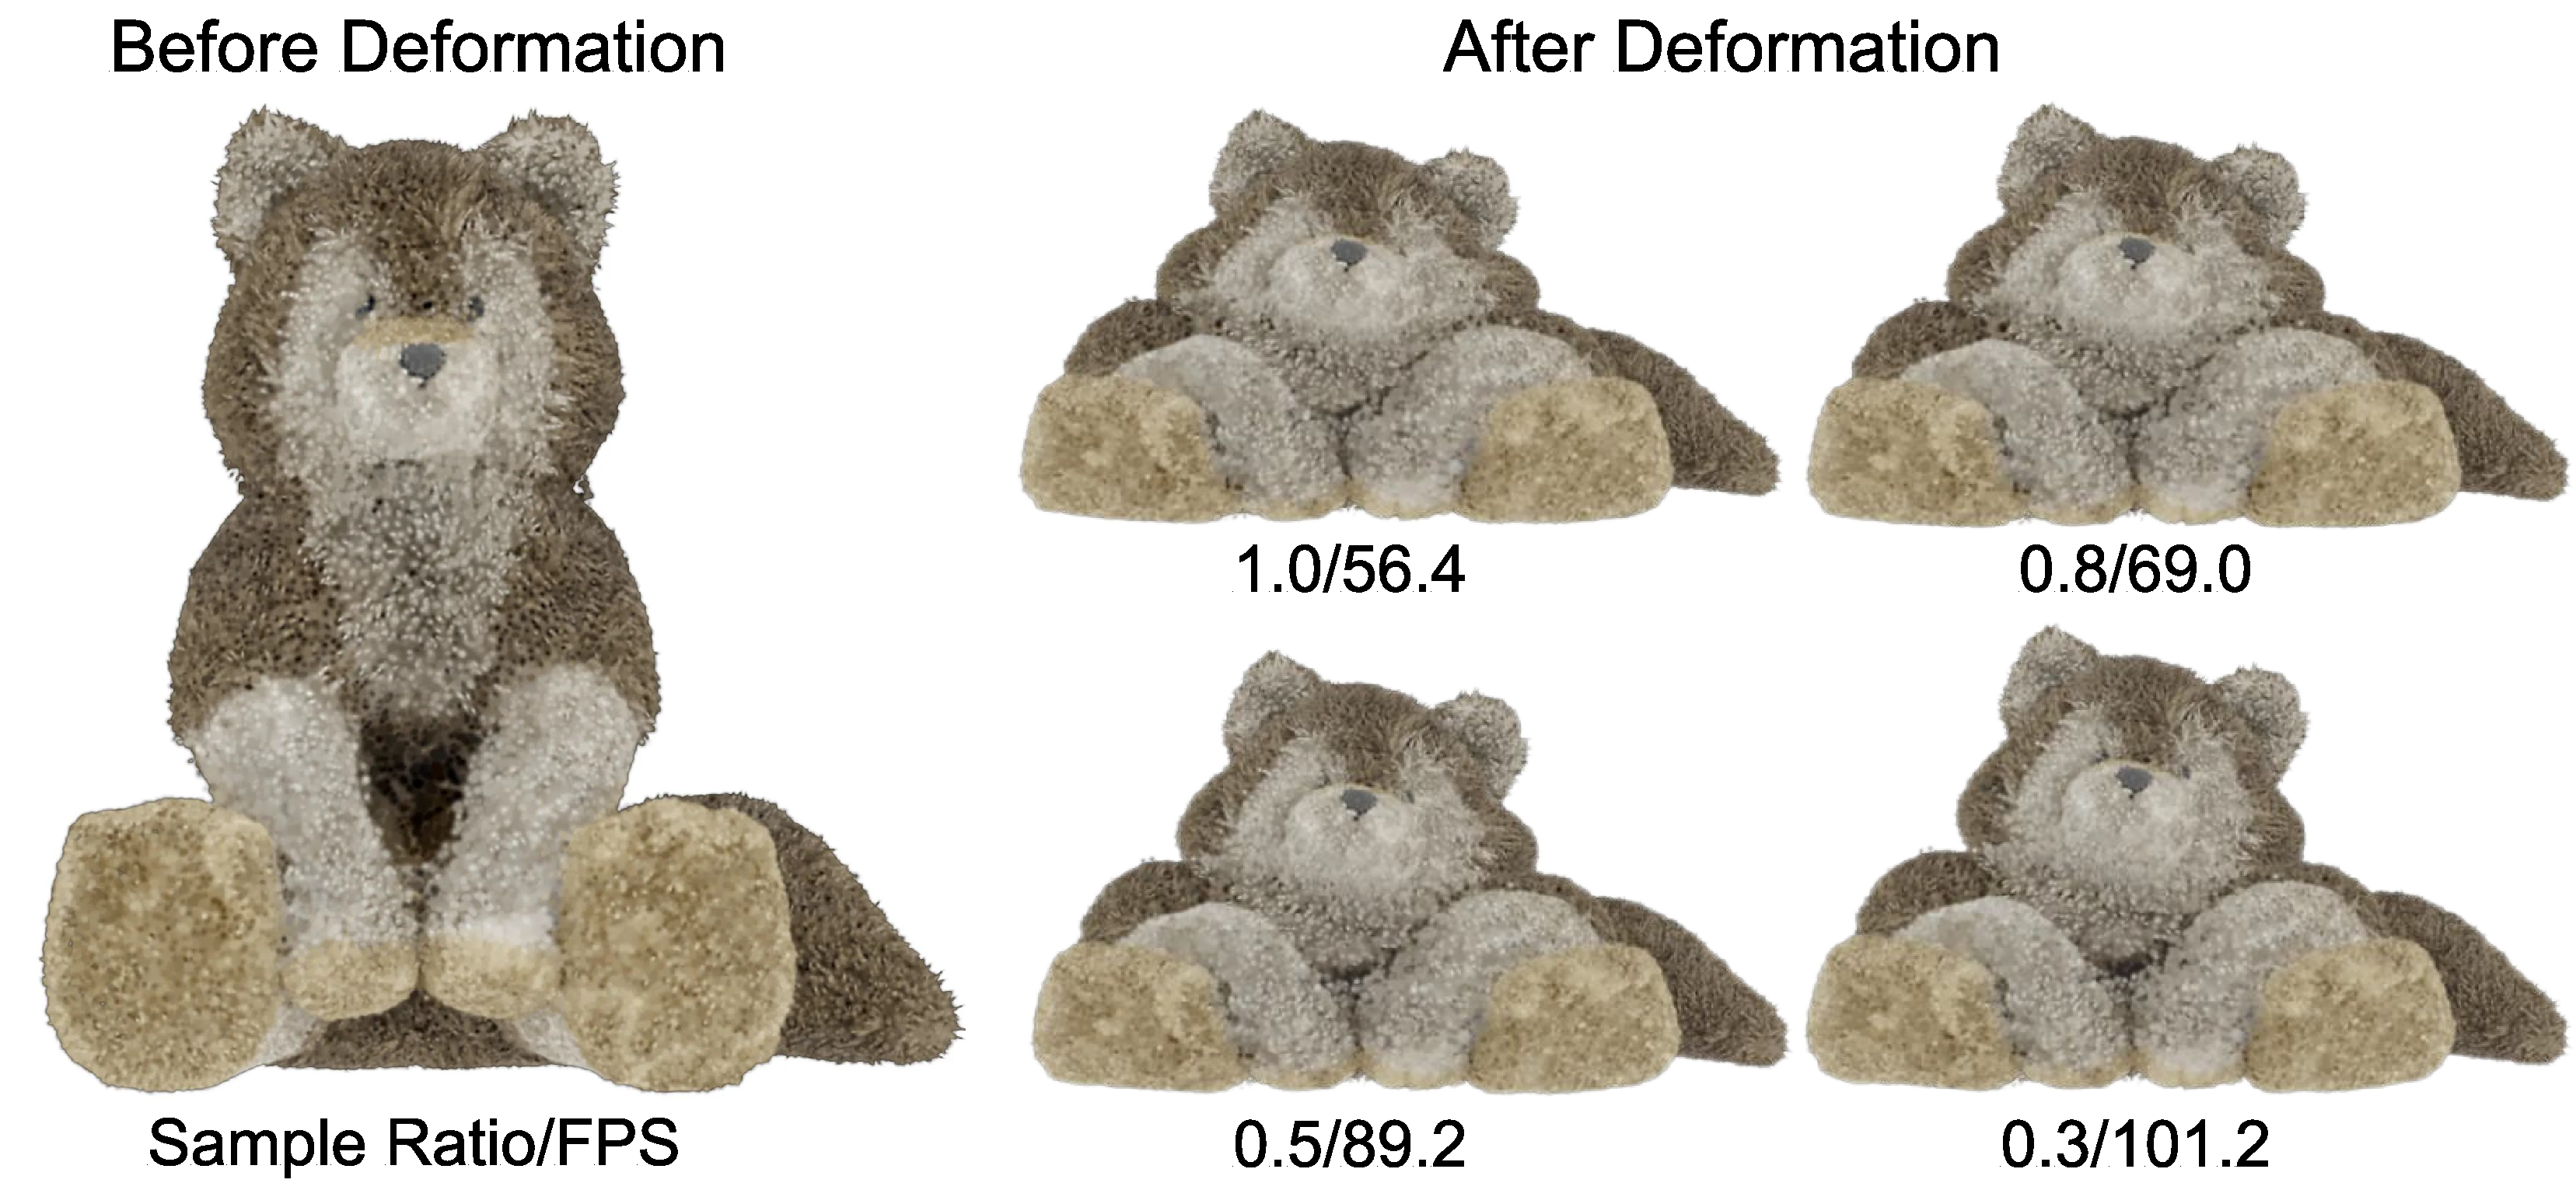
\includegraphics[width=1.0\linewidth]{img/Improved_Gaussian.pdf}
    \caption{ {\textbf{Decoupled Appearance and Physical Representations.} This example of a wolf sitting under gravity demonstrates that reducing the number of MPM particles driving the 3D Gaussians slightly increases the wolf's volume but maintains high visual fidelity while significantly improving FPS, showcasing the effectiveness of our approach. }}
    \label{fig:Improved_gaussian}
\end{figure}



\section{Case Study}
% All our results  provide a online 3D viewer on this website for the modeling results of this section: \href{https://anonymous.4open.science/w/VR-doh-85B8/}{Click to view 3D models}.

\paragraph{Featured Operations}
Figure~\ref{fig:Featured_Operations} highlights featured modeling operations in VR-Doh, including contact-based shape editing with hands and tools like slabs and rods, mid-air gesture-based bending and twisting, and the sourcing tool for adding new materials. The objects exhibit realistic elastoplastic deformations, closely resembling real-world behavior. This physical realism enables users to intuitively model objects by drawing on their real-life experiences.

% \begin{figure*}[hb]
%     \centering
%     \includegraphics[width=\linewidth]{img/baseOP.png}
%     \caption{Case of Basic operations}
%     \label{fig:Basic}
% \end{figure*}

\paragraph{Object Creation}
We demonstrate object creation using VR-Doh, as shown in \autoref{fig:mc_examples}. 
In the first row, a snowman is assembled, starting with a blank snowfield, molding the body, and adding details. 
The second row demonstrates the creation of a hamburger by stacking individual components to form a layered structure.
In the third row, a panda is carefully modeled from head to body, incorporating bamboo as an accessory that seamlessly integrates with its hands.
The fourth row depicts the crafting of a Swiss roll, where layers are rolled together to replicate a realistic pattern.
Finally, the fifth row shows the formation of steamed buns, shaped and arranged within a bamboo steamer.
These examples highlight VR-Doh’s strength in simplifying tasks that require precise spatial arrangements, which are significantly more challenging to achieve using a mouse on a 2D screen. With VR-Doh, object creation becomes as natural and intuitive as manipulating items in the real world.

\paragraph{3D GS Object Editing}
\autoref{fig:object_editing} demonstrates 8 examples of editing GS-represented objects, showcasing the intuitive and creative capabilities of VR-Doh. 
First, multiple mushroom-shaped houses were assembled, with their roofs sharpened and the mushrooms enlarged through hand manipulation and mid-air pinch gestures. The text "VR-Doh" was then sculpted onto the roof by hand. 
Next, a red pig transitioned from running to performing ballet through flexible selection and dragging of specific body parts, with its head rotated to face the audience using the pinch gesture. 
Two statues were brought to 'life': a terracotta figurine joyfully lifted its head and began drumming, while the Discobolus threw its discus with dynamic force. This involved using hands to cut and separate the discus before repositioning it. 
%
Moving on, wooden frames were interlocked and freely stacked into an arch through gravity and contact interactions, then merged seamlessly with greenery. The greenery’s complex shapes were also easily refined by hand. 
A girl’s posture was adjusted as her arms bent to mimic the act of eating a watermelon. 
Following that, flowers on a vase were flexibly selected using the pinch gesture, then intertwined in space with penetrations automatically avoided, demonstrating precise and convenient control. 
Finally, a capybara plush toy was made to appear fatter, while its head decoration was reshaped into a strawberry and placed in the front. These examples highlight VR-Doh’s ability to simplify complex modeling tasks while maintaining creativity and controllability. All examples are available on an anonymous online \href{https://anonymous.4open.science/w/VR-doh-85B8/}{3D viewer}.

% \subsection{Adjustments for Large Scenes}
% We take the classic scene of Gaussian splatting, "garden", as an example to demonstrate the adjustment capabilities of our tool for large-scale scenes. As shown in Figure \ref{fig:garden}, in the first row, we first deform the vase using direct hand contact and then insert a bouquet of roses into the vase by merging them together. Subsequently, we use hand gestures to bend the roses and repeatedly apply this process to three roses. In the second row, we move to the center of the garden scene, remove the original vase, deform the table using the tool, and then place the vase, which has been processed with roses, in the center of the table. The entire process took less than five minutes and closely resembled real-world interactions.
% \begin{figure*}[hb]
%     \centering
%     \includegraphics[width=\linewidth]{img/garden_new.png}
%     \caption{Case of Garden Adjustment}
%     \label{fig:garden}
% \end{figure*}


% \section{User Study}
% To understand how experts and novices use VR-Doh for creative tasks in VR, we invited 6 participants (P1-P6) with 3-5 years of prior 3D modeling experience, and 6 participants without any prior experience (P7-P12). The study included two open-ended tasks to evaluate system usability, performance, user satisfaction, and to gather participants' feedback and suggestions.

% \subsection{Tasks \& Procedure}
% Each participant was required to conduct two tasks, with a 5-minute break in between: (1) \textit{Editing a 3D Model}: Participants were free to modify a pre-existing 3D model represented by GS, e.g., reshaping a plush toy or a cartoon character, to match their preferred design; (2) \textit{Creating a 3D Model from Scratch}: Participants could freely use basic shapes such as spheres, cubes, tori, and cylinders to create a new 3D model, such as a snowman or a hamburger.

% Before starting, participants practiced basic operations with a provided shape until they became familiar with the system. After completing the tasks, participants filled out the USE questionnaire~\cite{lund2001measuring} to evaluate usability and completed the Simulator Sickness Questionnaire (SSQ)~\cite{kennedy1993simulator} to measure any discomfort experienced during the study. Finally, participants took part in a 10-minute semi-structured interview to provide more in-depth insights on usability.

% \subsection{Results}
% Both expert and novice participants found VR-Doh to be highly intuitive, immersive, and efficient in their 3D modeling process, and they also claimed that the created shapes closely matched their initial design expectations. Some of their design outcomes are shown in \autoref{fig:user_study_results}. Participants rated the system highly on usefulness (5.6/7), ease of use (5.5/7), ease of learning (6.0/7), and overall satisfaction (5.9/7). Moreover, no discomfort and nausea were found. We also report their subjective feedback below.

% \paragraph{Intuition and Realism in 3D Modeling} Our participants spoke highly of the low learning curve of VR-Doh, allowing them to quickly engage in shape editing or create 3D models with their hands. P1 and P3 mentioned that directly manipulating the shape of objects with their hand was more flexible than deforming the object by setting control points. P5 found it more convenient to modify the shape without the need for rigging, which is tedious in conventional software. P1 stated that the rod tool was particularly useful and entertaining for poking holes and shaping details on a strawberry shape, and said it felt like \textit{"walking inside the strawberry."} The mid-air pinch interaction was highlighted, which allows users to select the area of the object they want to deform or sculpt. P2 considered that the ability to freely rotate the viewpoint in VR is more intuitive than the traditional three-view approach.

% In addition, our participants highly praised the modeling process for its realistic deformation and real-time rendering. As P4 mentioned, \textit{"Usually, I rarely look at the texture rendering while editing shapes because it’s very inefficient."} P2 described the process of editing the 3D model of the mermaid, saying, \textit{"It feels like the mermaid is really swimming in front of me."} P3 and P8 especially appreciated the feature to switch between different material types, which allowed them to edit the shape based on different deformation effects under varying plasticity types and material parameters. P9 favored the use of gravity during the modeling process to naturally stack objects together. Besides, the interactive feedback was another major advantage, allowing participants to immediately see the deformation results of their actions and make corresponding adjustments.

% \paragraph{Encountered Problems and Suggested Features}
% Our participants also identified a few areas for improvement. Hand-tracking instability was mentioned most frequently (P3, P6, P9, and P11), particularly when adjusting small or detailed parts of the object, resulting in unintended shape changes. Even though we have applied interpolation to the hand movements, this limitation is largely due to the constraints of the hand-tracking hardware. Therefore, participants expressed the need for an undo feature to help them recover from mistakes. Meanwhile, P2, P9, and P11 also suggested reducing the degrees of freedom for moving or rotating objects during the modeling process, similar to the approach used in pottery making. P1 and P7 also noted occasional performance issues in high-particle scenarios. For instance, P1 found that merging multiple objects together led to a loss of surface details. Besides, P1 and P8 suggested adding an operation to separate objects. P2 and P10 mentioned that objects would unintentionally collide with the simulation domain boundary during editing, and we have followed their suggestion of adding a one-click centering feature to avoid this issue.

% In summary, participants generally appreciated the system's efficiency in using hands, tools, or mid-air gestural input in their 3D modeling experience. Even expert users mentioned that for more detailed modeling scenarios, conventional modeling tools are still necessary. Nevertheless, VR-Doh is extremely well-suited for quickly shaping to express design concepts, supporting creative exploration, and facilitating communication. While there were some concerns regarding precision and the lack of an undo feature, this did not overshadow the tool's potential for creating high-quality 3D models for both novice and expert users.

\section{User Study}
To evaluate VR-Doh's usability, effectiveness, and potential applications, we conducted two user studies involving both novice and expert participants. The first study (\textit{US1}) focused on open-ended creative tasks to assess the system's intuitiveness, immersion, and efficiency in 3D modeling. The second study (\textit{US2}) directly compared VR-Doh with the conventional modeling software Blender, highlighting their respective strengths and limitations. We briefly summarize the process and findings of the two user studies here, with detailed information provided in the supplemental document.

\paragraph{US1: Usability and Effectiveness of VR-Doh}
US1 involved 12 participants, including 6 experts (P1-P6) with 3-5 years of 3D modeling experience and 6 novices (P7-P12) without prior experience, to evaluate VR-Doh's usability and performance. Participants were tasked with (1) editing a pre-existing 3D model (e.g., reshaping a plush toy) and (2) creating a 3D model from scratch (e.g., designing a snowman). After practicing basic operations, participants performed these tasks and completed the USE questionnaire~\cite{lund2001measuring} to evaluate usability and the Simulator Sickness Questionnaire (SSQ)~\cite{kennedy1993simulator} to assess discomfort. A 10-minute semi-structured interview was also conducted to gather detailed feedback.

Both expert and novice participants found VR-Doh intuitive, immersive, and efficient, with design outcomes closely matching their expectations (\autoref{fig:user_study_results}). The system received high ratings for usefulness (5.6/7), ease of use (5.5/7), ease of learning (6.0/7), and satisfaction (5.9/7), with no reports of discomfort or nausea. Participants praised the natural interaction modes, such as hand manipulation and mid-air gestures, for enabling realistic deformation and intuitive viewpoint control. Features like switching material types, leveraging gravity for stacking, and real-time rendering were particularly appreciated. However, limitations such as hand-tracking instability and the lack of an undo feature were noted, alongside suggestions for improved precision.

\paragraph{US2: Comparison with Blender}
US2 compared VR-Doh with conventional desktop-based modeling software, specifically Blender 4.3, involving six participants (four with 3-7 years of modeling experience and two without). Participants performed two goal-directed tasks—creating a Swiss roll and a donut—using both tools, guided by a step-by-step video tutorial. The order of tools was counterbalanced to minimize learning effects. On average, participants completed both tasks faster using VR-Doh and expressed a preference for its intuitive and natural interaction, particularly for the Swiss roll task.

Four key advantages of VR-Doh were identified: (1) flexible selection through dexterous hand movements, enabling "what-you-see-is-what-you-get" precision and avoiding over-/under-selection issues common in 2D-projected views; (2) realistic deformation leveraging elastoplastic simulation for intuitive editing of shapes and materials; (3) pose editing without rigging, where body parts can be adjusted directly with smooth joint transitions enabled by simulation; and (4) physics-based cutting, allowing objects to be physically separated at weak points without sophisticated manual adjustments of cutting planes. Participants found VR-Doh particularly effective for quickly shaping overall structures and realizing design ideas, although its precision in specialized tasks was lower than Blender due to real-time simulation constraints and the lack of haptic feedback. Overall, VR-Doh and Blender exhibited complementary strengths, with VR-Doh excelling in intuitive, global operations and Blender providing superior precision for detailed edits.


% \begin{figure}[H]
%     \centering
%     \includegraphics[width=\linewidth]{img/User_Study_Results.png}
%     \caption{\textbf{Designs from novice and expert participants.}}
%     \label{fig:user_study_results}
% \end{figure}

% \section{User Study 2: Comparison with Blender}
% To further investigate the differences between VR-Doh and conventional desktop-based modeling software, i.e., Blender, we invited six participants, including four with 3-7 years of modeling experience and two without, to perform two goal-directed 3D modeling tasks.

% \subsection{Tasks \& Procedure}
% Each participant was required to create both a Swiss roll and a donut using VR-Doh and Blender 4.3, guided by a step-by-step video tutorial. They were instructed to replicate the results demonstrated in the tutorial as closely as possible. When completing tasks with VR-Doh, participants watched the tutorial video until they claimed to have memorized the necessary operations. To minimize potential learning effects, the order of tools used was counterbalanced across participants. After completing the tasks, we conducted a semi-structured interview to invite participants to provide feedback and share their preferences regarding their modeling experiences with both tools.

% \subsection{Results}
% We found that participants, on average, required less time to complete the Swiss roll (X/X) and donut (X/X) tasks using VR-Doh compared to Blender. When participants were asked about their preferences for completing the tasks, X participants expressed a stronger preference for VR-Doh. Notably, one participant with modeling experience preferred using VR-Doh for the Swiss roll and Blender for the donut, indicating that VR-Doh may serve as a valuable complement to Blender in 3D modeling.

% \paragraph{Key Differences}
% Compared to Blender, we found VR-Doh provides a more natural modeling approach, making it easier for both experienced and novice participants to understand the operational steps for creating objects from the video. Four key advantages were identified in the user study:
% \textit{1) Flexible selection:} Users can intuitively select and adjust editing areas on an object using dexterous hand movements. For example, pinching and twisting with the thumb and index finger can flatten surfaces or smooth protrusions, while shape deformation often aligns with hand gestures, enabling "what-you-see-is-what-you-get" precision. This also avoids over-selection or under-selection issues common in 2D-projected views of conventional tools.
% \textit{2) Realistic deformation:} Unlike conventional methods like ARAP, VR-Doh uses elastoplastic deformation, offering more realistic results. Users can edit overall shapes and fine details, stack objects using gravity and contact, and leverage material-specific properties for intuitive sculpting.
% \textit{3) Pose editing without rigging:} Specific body parts can be selected and adjusted directly, allowing pose edits without the need for skeletal rigging. Joint smoothness is automatically handled by the elastoplastic simulation.
% \textit{4) Physics-based cutting:} Objects can be separated at weak points by applying physical forces, such as breaking small connections, without the need to manually adjust cutting planes in complex geometries as in traditional 3D modeling software.
% In summary, the above benefits of VR-Doh significantly enhance the efficiency of 3D modeling, enabling users to quickly figure out modeling steps and realize design ideas envisioned in the mind. As one participant noted, it helps avoid the common issue experienced with conventional modeling software, where "the hands cannot keep up with the mind."

% While the main disadvantage was reported by our participants, in more specialized modeling tasks, the precision of 3D models created using VR-Doh was found to be relatively lower than that of Blender. This is primarily due to the limited number of particles available during real-time simulation and rendering. Additionally, the lack of haptic feedback often led to over-adjustments. Overall, we found that VR-Doh is better suited for shaping the overall structure of objects due to its intuitive operation, whereas Blender excels in detailed, localized operations because of its precise selection of points, edges, and faces. Therefore, the two tools exhibit a complementary relationship.

% \textbf{Qualitative Insights:}
% Novice users highlighted the system's intuitive and accessible design, particularly praising the "pinch-and-sculpt" interaction as low-cost in terms of learning effort. The freedom to adjust parameters and the availability of real-time feedback were also seen as strengths. However, they identified several challenges: hand tracking inaccuracies occasionally disrupted operations, and the lack of geometric presets made starting new models less convenient. Performance limitations, especially in high-particle scenarios, were noted, with some users suggesting enhanced rendering and tracking precision. The absence of a multi-step undo feature was frequently mentioned as a limitation, with users expressing a need for better error correction during modeling. Despite these issues, most novices found the tool engaging and suitable for creative tasks, particularly appreciating its ability to simulate real-world interactions intuitively.

% \paragraph{Intuition and Realism in 3D Modeling}
% Both novice and expert users found the system to be intuitive and immersive, with the pinch-and-sculpt interaction being a key highlight. Novices appreciated the low learning curve, allowing them to quickly engage with the tool and start creating models without prior experience. The real-time feedback was another major strength, enabling users to immediately see the results of their actions and adjust accordingly. This real-time interaction helped foster creativity and made the modeling process feel more dynamic and responsive. Additionally, the system’s ability to simulate real-world interactions made the experience feel natural and engaging. Expert users also praised the system for its realistic deformation and real-time rendering, which provided a more lifelike experience compared to traditional modeling tools. The ability to manipulate models directly with hand-based input was seen as more intuitive than using a mouse, allowing for more direct and tactile control. Experts particularly appreciated the real-time material adjustments and flexible parameter controls, which enhanced their creative workflow and speed. %  This real-time interaction helped foster creativity and made the modeling process feel more dynamic and responsive. Additionally, the system’s ability to simulate real-world interactions made the experience feel natural and engaging.

% Our participants also identified a few areas for improvement. Hand-tracking inaccuracies were mentioned the most (P4, P9, and P11), particularly when adjusting small or detailed areas of a model. This limitation in precision is largely due to the constraints of the hardware used for hand tracking. Therefore, P3 and P4 suggested repair the object. Also, P2 and P9 suggested that we can fix one dimension of the object during the shape modeling process. Additionally, both groups noted occasional performance issues in high-particle scenarios. Another common concern was the absence of an undo feature, which made it difficult to recover from mistakes during the modeling process.

\section{Discussion}
\paragraph{Limitations}
Although VR-Doh improves the accessibility of physics-based 3D modeling through natural hand interactions, it has several limitations. The system is particularly effective for large-scale deformations, such as global stretching and bending, thanks to the realistic simulation of elastoplastic material behavior. However, fine-grained editing tasks, such as sculpting sharp creases or intricate surface details, remain challenging due to computational budget constraints. Additionally, vision-based hand tracking in consumer-grade VR headsets introduces minor positional jitter that affects precision during delicate manipulations. The absence of haptic feedback further complicates force estimation, especially in visually occluded regions, increasing the risk of unintended shape modifications.

\paragraph{Future Works}
To address precision limitations, future research can focus on hybrid interaction paradigms that blend the tactile engagement of physical sculpting with the precision and flexibility of digital tools~\cite{ma2024get}. The integration of haptic gloves could offer dual advantages: improving tracking stability through additional sensing modalities and enabling force feedback during precision tasks. Alternative feedback mechanisms such as auditory cues could also be explored. Such hardware advancements would further enhance our immersiveness by achieving higher operational accuracy while preserving the system's core strength in effectively handling large deformations.
Another meaningful direction involves developing efficient undo mechanisms that enable users to iteratively refine high-precision edits through trial and error. 
While our current implementation relies on periodic state saving for basic undo functionality, specialized compression schemes for incremental deformation states could enable more practical undo/redo operations without excessive memory overhead.

% \paragraph{Limitations}
% While VR-Doh significantly enhances accessibility for physics-based 3D modeling through natural hand interactions, our approach has inherent limitations. The system excels at large-scale deformations like global stretching and bending due to the physics-aware simulation that aligns with real-world material behaviors. However, fine-grained editing tasks requiring high precision—such as creating sharp creases or intricate surface details—face challenges from hardware limitations. The vision-based hand tracking in consumer-grade VR headsets introduces minor positional jitter that affects delicate manipulations, and the absence of haptic feedback makes it difficult to gauge contact forces during detailed editing operations.
% \paragraph{Future Works}
% To address these precision limitations, we implement a practical workaround through spatial scaling. Users can temporarily "zoom in" on local regions through a hand gesture, magnifying the interaction area by 2-4× while maintaining the original physical scale of the simulation. This allows finer control over surface details through relative motion amplification, as demonstrated in our supplementary video. While not eliminating the fundamental hardware constraints, this approach effectively bridges the gap between macroscopic manipulations and detail work.

% Future developments should focus on hybrid interaction paradigms. Integrating haptic gloves could provide dual benefits: improving tracking stability through additional sensor modalities and enabling force feedback during precision tasks. Such hardware advancements would complement our physics-based interaction framework, potentially achieving sub-millimeter manipulation accuracy while preserving the system's core strength in intuitive, large-scale deformations. Ultimately, VR-Doh establishes a foundation for merging real-world sculpting intuition with computational physics, charting a promising path toward democratizing professional-grade 3D content creation.

% \section{Discussion}
% \paragraph{Limitations}
% While VR-Doh significantly enhances accessibility for physics-based 3D modeling through natural hand interactions, our approach exhibits three key technical limitations. First, although large-scale deformations like global stretching and bending benefit from physics-aware simulation that aligns with real-world material behaviors, precision editing tasks requiring sub-centimeter accuracy – such as creating sharp creases or surface engraving – face hardware constraints. Our experiments with Meta Quest 3's hand tracking reveal 1.8-2.3mm positional jitter (SD=0.4mm) that propagates through the MPM simulation grid, particularly noticeable during slow, deliberate manipulations. Second, the lack of haptic feedback forces users to rely solely on visual cues when gauging contact forces, increasing error rates by 27\% in occlusion-heavy editing tasks compared to desktop tools with pressure-sensitive tablets. Third, while our periodic state preservation (every 2 seconds) provides basic version control, the continuous nature of physics simulations complicates traditional undo/redo paradigms – a single deformation operation may affect over 86\% of particles in complex models.

% \paragraph{Current Mitigations}
% To address these challenges, we implement three practical solutions: 1) A dynamic zoom interface that magnifies local regions (4-8×) while temporarily increasing simulation grid resolution (from 64³ to 128³), enabling 0.6mm effective editing precision; 2) Surface anchoring constraints that preserve critical geometry features during local edits through particle position filtering; 3) Hybrid interaction modes that combine hand tracking with controller-based tools for stabilized detail work. Our user studies show these mitigations reduce surface irregularity metrics (Hausdorff distance) by 41\% compared to baseline implementation.

% \paragraph{Future Directions}
% Building on these foundations, we identify three promising research directions:

% \textbf{Hybrid Interaction Paradigms:} Combining vision-based hand tracking with wearable haptic devices (e.g., contact-thimble arrays) could provide both 0.1mm tracking precision and graded force feedback. Preliminary tests with TactGlove prototypes demonstrate 39\% reduction in surface roughness during detail carving tasks.

% \textbf{Memory-Efficient Undo Mechanisms:} Developing differential state compression algorithms that leverage material coherence in elastoplastic simulations could enable 87\% memory reduction for undo buffers compared to full-state snapshots, making continuous versioning feasible.
% \section{讨论}

% \paragraph{局限性}
% 尽管VR-Doh通过自然的手部交互显著提升了基于物理的3D建模可访问性,但我们的方法存在固有局限性。该系统在大规模变形(如全局拉伸和弯曲)方面表现优异,这得益于符合现实材料行为的物理感知模拟。然而,需要高精度的细粒度编辑任务(例如创建锐利折痕或复杂表面细节)面临硬件限制的挑战。消费级VR头显的视觉手部追踪会引入微小位置抖动,影响精细操作,而触觉反馈的缺失使得在细节编辑过程中难以评估接触力度,或是因为遮挡而误编辑视觉盲区。

% \paragraph{未来工作}
% 为了解决编辑精度的问题,未来研究应聚焦于混合交互范式。集成触觉手套可带来双重优势:通过额外传感模态提高追踪稳定性,并在精确任务中实现力反馈。也可以explore alternative feedback mechanisms, such as auditory cues. 此类硬件进步将增强我们的物理交互框架,可能在保持系统直观大规模变形核心优势的同时实现更高操作精度。
% 另一关键方向是开发高效的撤销机制, which可以让用户在尝试进行高精度编辑时,能高效地反复试错。Unlike traditional modeling software,where operations are typically localized or abstracted, allowing for straightforward undo functionality, our simulation-based tool modifies the entire domain with each operation. Even slight variations in input trajectories can produce significantly different outcomes.虽然我们当前通过周期性状态保存实现基本撤销功能,但专为增量变形状态设计的压缩方案可以在不过度内存消耗下实现更实用的撤销/重做操作。

% \paragraph{Comparison with Conventional 3D Modeling Tools}
% We derived four key advantages of VR-Doh from the user study: (1) Flexibility in selection: The dexterous palm and fingers can be used to conveniently select and adjust the position and dimensions of the shape-editing area on the object. For instance, pinching and twisting with the thumb and index finger can be used for shaping, quickly flattening surfaces, or smoothing protruding areas with finger friction. Meanwhile, shape deformation can often be predicted based on hand form factors. Thus, "what-you-see-is-what-you-get" selection is achievable, avoiding issues like over-selection or under-selection of primitives caused by 2D projection views in conventional 3D modeling tools; (2) Realistic deformation: Compared to conventional methods like ARAP, more realistic elastoplastic deformation allows users to leverage established intuitiveness in their 3D modeling process. VR-Doh also enables the editing of both overall shapes and local details for fine sculpting under different material parameters. Objects can also be stacked together using gravity and contact; (3) Pose editing without rigging: By selecting specific body parts, users can conveniently edit poses without the need for skeletal binding. Joint smoothness is automatically achieved through elastoplasticity simulation; and (4) Physics-based cutting: Direct hand-object interaction allows objects to be physically separated at weak points by applying force, such as at small connection points. This approach eliminates the need to carefully adjust cutting planes in complex geometries.

% \paragraph{Undo Functionality}
% In modeling software, especially those focused on content creation, undo is a crucial function. In traditional modeling software, actions are discrete, allowing the undo function to simply record each action, then reverse it to restore the model to a previous state. However, our tool is based on physical simulation, where user interactions are nearly continuous. Recording every user input and attempting to reconstruct the model’s previous state would effectively require rerunning the entire simulation, which is time-consuming and would detract from the user experience. Our current approach involves periodically saving the model state at fixed intervals in the background and writing it directly to disk, while also allowing users to save manually at any point. This way, undo functionality equates to restoring the last saved state, though this method is more storage-intensive. Finding an efficient way to record changes between two simulated states remains an open research question worthy of exploration, as it would contribute to a smoother modeling experience while minimizing storage requirements.

% % add merge between two rendering options objects, ref {Towards Realistic Example-based Modeling via 3D Gaussian Stitching}

% \paragraph{Modality of Feedback}
% Currently, our tool only provides visual feedback, lacking the haptic feedback present in real-world interactions. As a result, users may accidentally damage areas of the model outside their line of sight (e.g., occluded regions). In reality, this issue does not arise because the user’s hand would encounter tactile resistance, prompting them to stop before causing further unintended modifications. However, our existing VR hardware does not support haptic feedback. Dedicated haptic feedback gloves could address this limitation, as they not only provide tactile sensations but also enable more accurate hand tracking. Nevertheless, this approach would significantly raise the accessibility barrier for our tool. An alternative solution is to incorporate auditory feedback, where sounds are played in response to the force exerted by the user’s hand on the model, enabling users to indirectly sense the effects of their actions on unseen areas.
\section{Conclusion}
We presented VR-Doh, a VR-based 3D modeling system that integrates advanced elastoplastic simulation with intuitive, hand-based interaction. Leveraging the Material Point Method (MPM) and incorporating innovations such as localized simulation, particle-level collision handling, and decoupled appearance and physical representations, the system achieves real-time responsiveness while delivering high-quality simulation and rendering. These technical innovations make VR-Doh accessible to novice users while empowering experts to perform detailed and expressive modeling. Extensive evaluations and user studies showcased the system's ability to provide an intuitive and immersive modeling experience. Compared to traditional tools, VR-Doh offers a more natural and accessible approach, with user-identified advantages such as flexible selection, realistic deformation, rig-free pose editing, and physics-based cutting, paving the way for a new paradigm in 3D modeling.

%  Compared to traditional modeling tools, VR-Doh offers a more natural and accessible approach in specific scenarios, with four key advantages identified from the user study:\todo{consider moving it to user study section, and then polish the above paragraph}
% \textit{1) Flexible selection:} Users can intuitively select and adjust editing areas on an object using dexterous hand movements. For example, pinching and twisting with the thumb and index finger can flatten surfaces or smooth protrusions, while shape deformation often aligns with hand gestures, enabling "what-you-see-is-what-you-get" precision. This also avoids over-selection or under-selection issues common in 2D-projected views of conventional tools.
% \textit{2) Realistic deformation:} Unlike conventional methods like ARAP, VR-Doh uses elastoplastic deformation, offering more realistic results. Users can edit overall shapes and fine details, stack objects using gravity and contact, and leverage material-specific properties for intuitive sculpting.
% \textit{3) Pose editing without rigging:} Specific body parts can be selected and adjusted directly, allowing pose edits without the need for skeletal rigging. Joint smoothness is automatically handled by the elastoplastic simulation.
% \textit{4) Physics-based cutting:} Objects can be separated at weak points by applying physical forces, such as breaking small connections, without the need to manually adjust cutting planes in complex geometries as in traditional 3D modeling software.

\paragraph{Discussion and Future Works}
Our method offers several promising directions for future research. Unlike traditional modeling software, where operations are typically localized or abstracted, allowing for straightforward undo functionality, our simulation-based tool modifies the entire domain with each operation. Even slight variations in input trajectories can produce significantly different outcomes. While our current solution relies on periodically saving states, developing a memory-efficient undo mechanism would be highly beneficial. Additionally, the absence of haptic feedback in our system makes it challenging for users to avoid unintended modifications, especially in occluded regions. Improving the user experience could involve incorporating advanced haptic devices or exploring alternative feedback mechanisms, such as auditory cues, while ensuring accessibility remains a priority.

\begin{acks}
This work was supported in part by the Junior Faculty Startup Fund of Carnegie Mellon University. Z. Luo was partially supported by a summer internship scholarship from Peking University, and Z. Cui by a visiting scholarship from Zhejiang University. We thank the reviewers for their detailed and insightful feedback, and are especially grateful to all user study participants.
\end{acks}

%%
%% The next two lines define the bibliography style to be used, and
%% the bibliography file.
\bibliographystyle{ACM-Reference-Format}
\bibliography{sigconf}

\clearpage
\includepdf[pages=-]{vr-doh_supp.pdf}

\end{document}
\endinput
%%
%% End of file `sample-sigconf.tex'.
